

\title{Arthromoteur : Attelle de mobilité passive continue du genou }
\maketitle
\begin{figure}[!h]
\centering
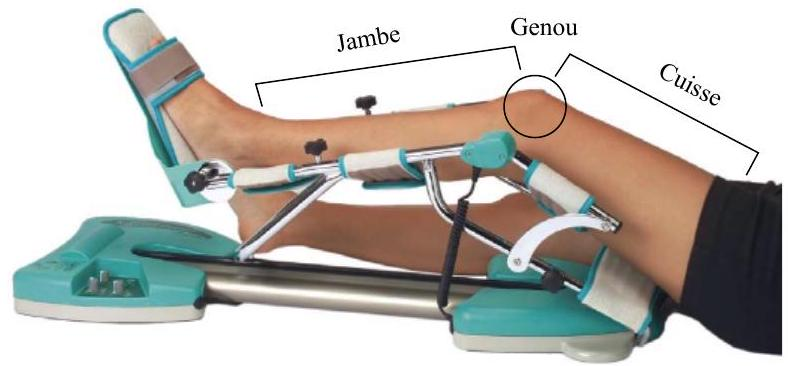
\includegraphics[max width=.5\textwidth]{2024_07_14_a83aebba33898893d39fg-01}

\caption{\label{fig:ccs_mp_2024:fig:01} Vue de l'arthromoteur en phase d'utilisation}
\end{figure}

\section{Mise en situation et problématique}
\subsection{Présentation générale}
Une arthroplastie du genou (intervention chirurgicale consistant à remplacer tout ou partie de l'articulation) est suivie d'une phase de rééducation post-opératoire dont les objectifs au niveau de l'articulation opérée sont de traiter la douleur, de diminuer l'inflammation, de relancer la vascularisation (circulation sanguine) et de récupérer la mobilité articulaire.

La société Kinetec a développé un arthromoteur automatisé destiné à la rééducation du genou (figure \ref{fig:ccs_mp_2024:fig:01}). Cet arthromoteur peut être utilisé en mode passif ou bien en mode actif.

L'étude proposée sera limitée au mode passif qui vise à récupérer la mobilité du point de vue de l'amplitude du mouvement du genou. La rééducation en Mobilisation Passive Continue (MPC) consiste en une succession de mouvements de flexion et/ou d'extension exécutés pendant une durée longue et sans que le patient soit acteur des mouvements. Le patient est passif et ses membres sont mis en mouvement par l'arthromoteur automatisé, le patient n'exerce aucun effort volontaire avec sa jambe et sa cuisse.

Au delà de l'intérêt thérapeutique de l'arthromoteur automatisé, les avantages de ce système sont sa portabilité et sa simplicité d'utilisation. Ainsi, le patient peut bénéficier de cette rééducation à domicile (présence postopératoire en établissement de soin réduite) et de façon autonome une fois sorti de l'hôpital.

\subsection{Contexte de l'étude}
L'arthromoteur automatisé peut être utilisé dans le cadre de nombreuses pathologies du genou. Ainsi, à l'aide du pupitre de commande (figure \ref{fig:ccs_mp_2024:fig:02}), le thérapeute peut choisir la valeur de plusieurs paramètres en fonction du protocole de la rééducation.

\begin{figure}[!h]
\centering
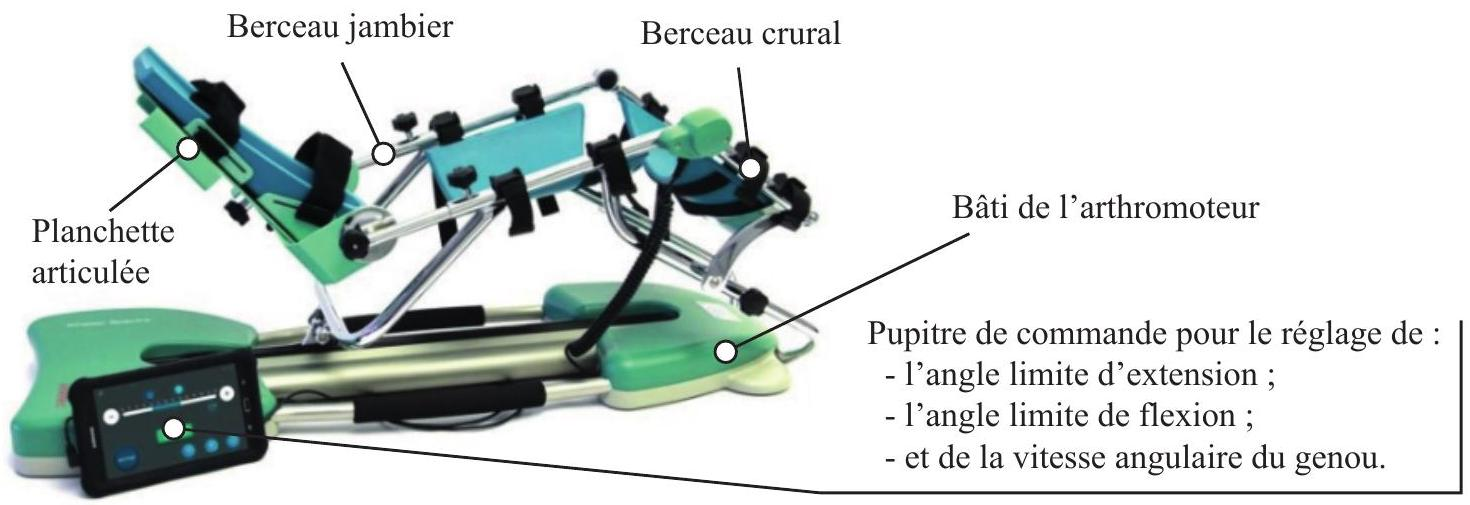
\includegraphics[max width=.8\textwidth]{2024_07_14_a83aebba33898893d39fg-01(1)}
\caption{\label{fig:ccs_mp_2024:fig:02}Architecture générale de l'arthromoteur}
\end{figure}
Dans le cadre de cette étude on se limitera aux trois paramètres du tableau \ref{tab:ccs_mp_2024:tab:01}, voir aussi la figure \ref{fig:ccs_mp_2024:fig:03}.

\begin{table}[!h]
\centering
\begin{tabular}{ll}
 & \textbf{Valeurs possibles} \\
\hline
Angle limite d'extension du genou & Jusqu'à $-5^{\circ}$ \\
Angle limite de flexion du genou & Jusqu'à $110^{\circ}$ \\
Vitesse angulaire constante du genou & De $50^{\circ}$ à $240^{\circ}$ par minute \\
\hline
\end{tabular}
\caption{\label{tab:ccs_mp_2024:tab:01}Valeurs possibles des paramètres réglables}
\end{table}



\begin{figure}[!h]
\centering
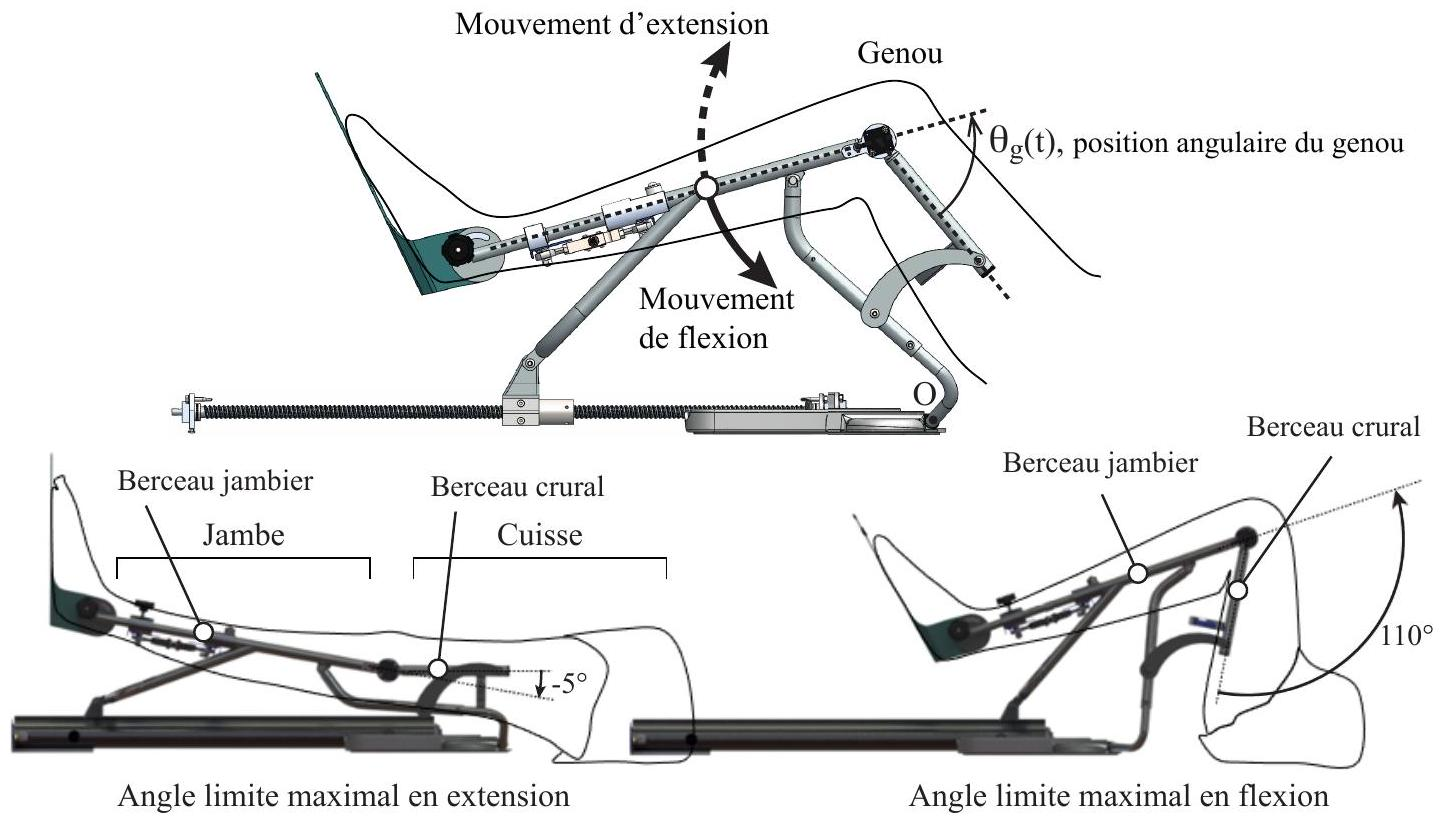
\includegraphics[max width=.8\textwidth]{2024_07_14_a83aebba33898893d39fg-02}
\caption{\label{fig:ccs_mp_2024:fig:03}Angles limites possibles en flexion et en extension avec l'arthromoteur}
\end{figure}

L'étude proposée par la suite sera réalisée dans le cadre d'une rééducation du genou après une reconstruction des ligaments croisés. Le protocole de rééducation des ligaments croisés impose une amplitude de mouvement du genou de $50^{\circ}$ avec un angle limite d'extension de $35^{\circ}$, un angle limite de flexion de $85^{\circ}$ et une consigne de vitesse angulaire du genou de $240^{\circ}$ par minute. L'ensemble des exigences de ce type de rééducation est fourni dans le diagramme des exigences en annexe.

\begin{obj}
L'objet de l'étude est d'évaluer les solutions retenues pour assurer une rééducation autonome du genou après une reconstruction des ligaments croisés, en mode passif, à l'aide d'un arthromoteur automatisé en respectant les exigences thérapeutiques.
\end{obj}

\subsection{Génération de la consigne de mouvement du genou pour le protocole de la rééducation des ligaments croisés}

\begin{obj}
Montrer que les informations de réglage fournies par le thérapeute ou le patient sont suffisantes pour établir une loi de consigne angulaire du genou conforme au protocole de la rééducation des ligaments croisés.
\end{obj}

Pour utiliser l'arthromoteur automatisé, le patient s'allonge au sol, pose sa cuisse sur le berceau crural de l'appareil et sa jambe sur le berceau jambier (figures \ref{fig:ccs_mp_2024:fig:01} et \ref{fig:ccs_mp_2024:fig:03}). Grâce au pupitre de commande, le thérapeute ou le patient règle l'angle limite de flexion, celui d'extension ainsi que la vitesse de rotation du genou (figures \ref{fig:ccs_mp_2024:fig:02} et \ref{fig:ccs_mp_2024:fig:04}). Une fois les réglages effectués, l'arthromoteur automatisé provoque le déplacement alternatif de flexion puis d'extension du genou en marquant une pause entre ces deux mouvements.

\subsubsection*{Notations }
\begin{itemize}
  \item Les trois informations de réglage fournies par le thérapeute ou le patient:
\begin{itemize}
  \item $\theta_{i}$ angle limite d'extension du genou $\left(\mathrm{en}^{\circ}\right.$ ) ;

  \item $\theta_{f}>\theta_{i}$ angle limite de flexion du genou (en ${ }^{\circ}$ );

  \item $\omega_{0}$ amplitude de la vitesse angulaire du genou $\left(\mathrm{en}^{\circ} \cdot \mathrm{min}^{-1}\right.$ ) ;
  \end{itemize}

  \item Le mouvement angulaire réel du genou :
\begin{itemize}
  \item $\theta_{g}(t)$ angle du genou (en radians) (figure \ref{fig:ccs_mp_2024:fig:03}) ;

  \item $\omega_{g}(t)=\dot{\theta}_{g}(t)$ vitesse angulaire du genou (en rad$\cdot \mathrm{s}^{-1}$ ) avec $\omega_{g}>0$ en flexion et $\omega_{g}<0$ en extension;
  \end{itemize}
  \item Les grandeurs de consigne de l'arthromoteur automatisé :
\begin{itemize}
  \item $\indice{\theta}{g c}(t)$ consigne angulaire du genou (en radians) ;

  \item $\indice{\omega}{g c}(t)=\dot{\theta}_{g c}(t)$ consigne de vitesse angulaire du genou $\left(\mathrm{en}^{\circ} \cdot \mathrm{min}^{-1}\right.$ );
  \end{itemize}
  \item Contrainte thérapeutique :
\begin{itemize}
  \item $\indice{\ddot{\theta}}{g c m}=$ constante $\left(\mathrm{en}^{\circ} \cdot \min ^{-2}\right.$ ) accélération-décélération angulaire maximale du genou retenue pour établir le profil de consigne figure \ref{fig:ccs_mp_2024:fig:05}.
\end{itemize}
\end{itemize}

\begin{figure}[!h]
\centering
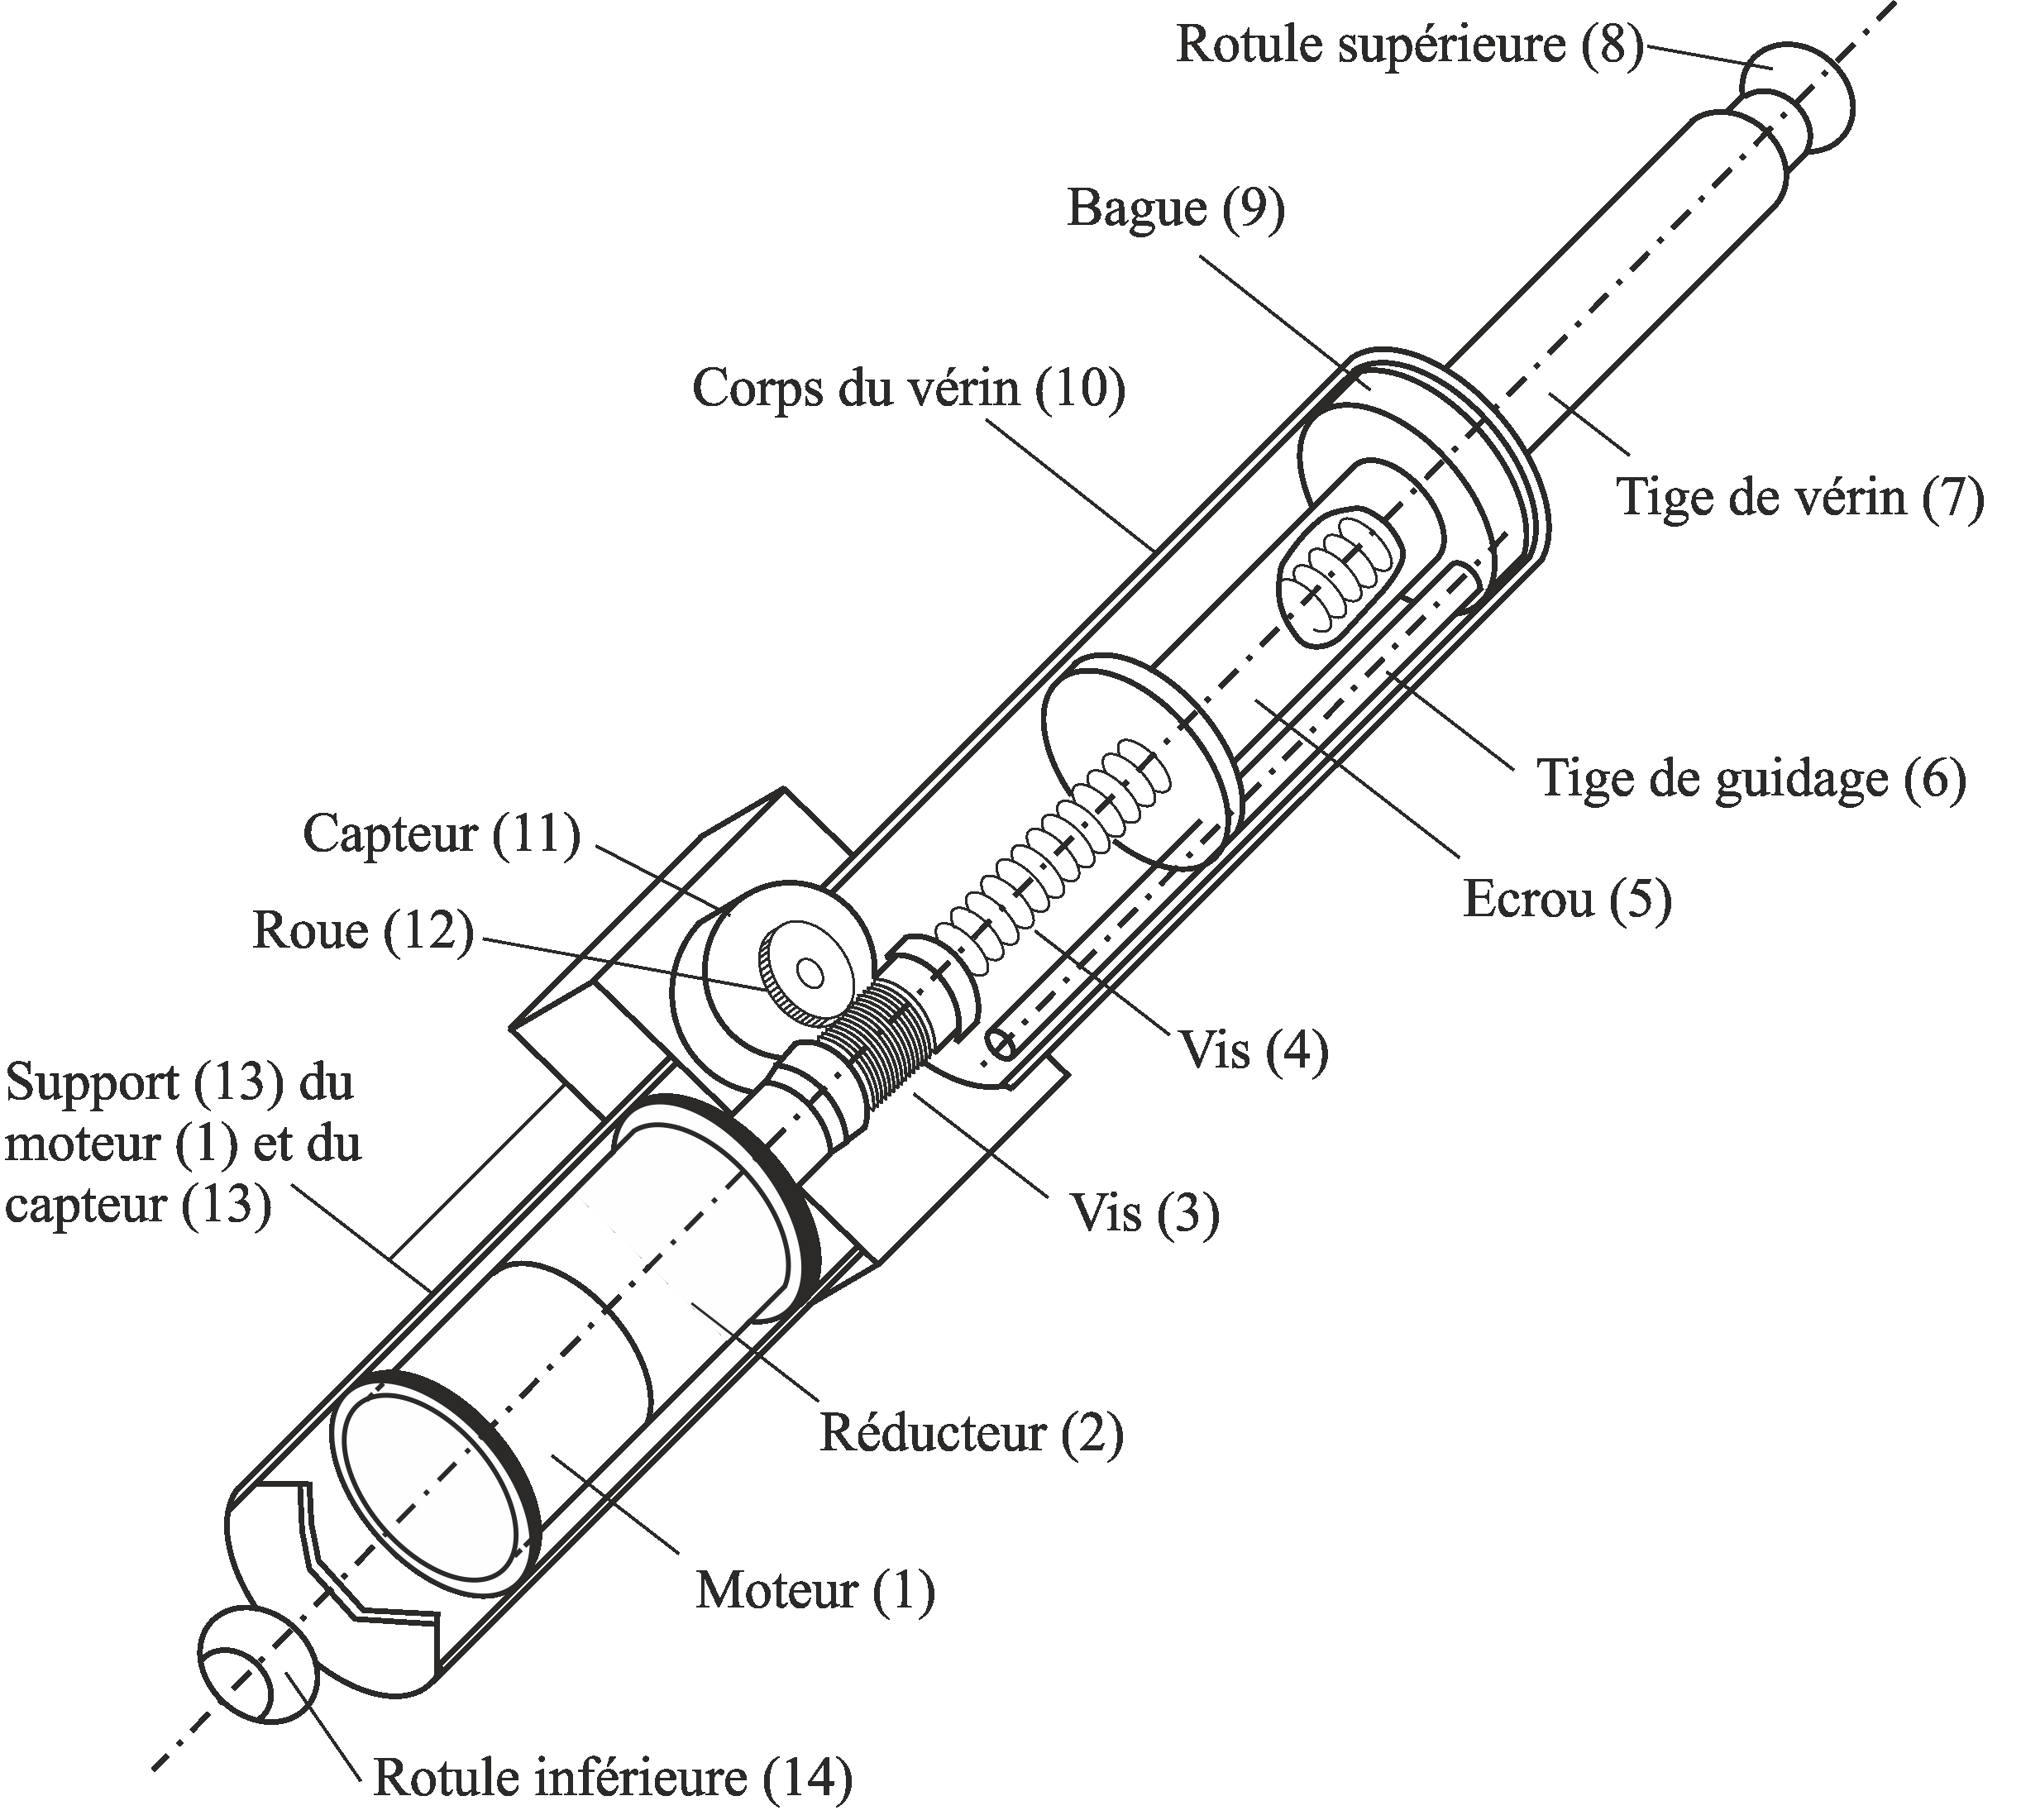
\includegraphics[width=\textwidth]{fig_04}
\caption{\label{fig:ccs_mp_2024:fig:04}Principe de la génération de la consigne angulaire du genou}
\end{figure}


%% \caption{\label{fig:ccs_mp_2024:fig:04}Principe de la génération de la consigne angulaire du genou}

D'un point de vue thérapeutique, il est nécessaire de limiter l'accélération-décélération du genou (voir id 1.1.1 du diagramme des exigences en annexe). Ce paramètre n'est pas réglable par le thérapeute.

La figure \ref{fig:ccs_mp_2024:fig:05} représente le profil de la consigne de vitesse angulaire du genou conforme au protocole de la rééducation des ligaments croisés.

\begin{figure}[!h]
\centering
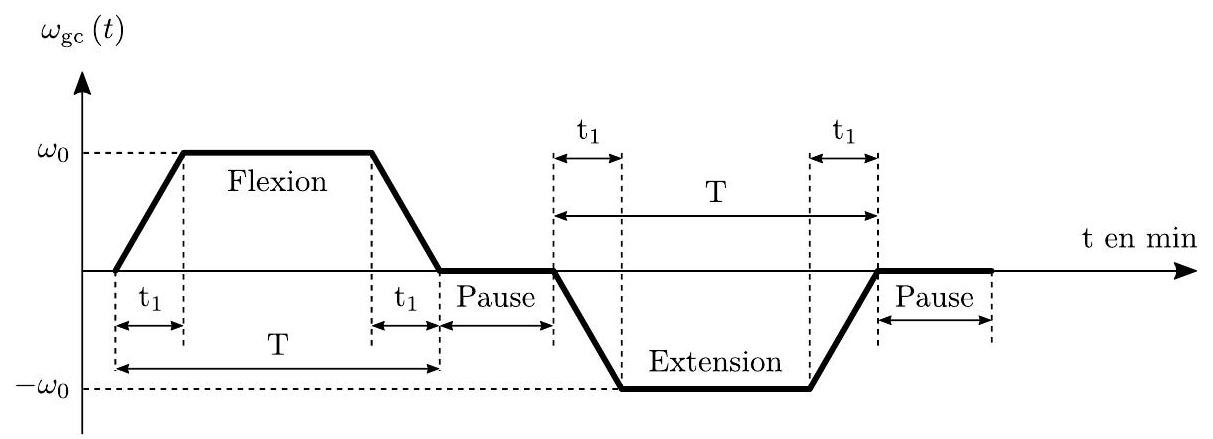
\includegraphics[max width=\textwidth]{2024_07_14_a83aebba33898893d39fg-03}
\caption{\label{fig:ccs_mp_2024:fig:05}Profil de consigne de vitesse angulaire du genou}
\end{figure}
Les durées des deux pauses sont supposées définies.

%Q 1. 
\question{ \label{q:ccs_mp_2024:01}Montrer que les informations de réglage fournies par le thérapeute ou le patient (figure \ref{fig:ccs_mp_2024:fig:04}) permettent d'établir une loi de consigne angulaire $\omega_{g c}(t)$ (figure \ref{fig:ccs_mp_2024:fig:05}) conforme au protocole de la rééducation des ligaments croisés. Pour cela, exprimer les durées $T$ et $t_{1}$ en fonction des quatre entrées du générateur de consigne angulaire du genou rappelées ci-dessous :}
\begin{itemize}
\item $\theta_{i}, \theta_{f}, \omega_{0} ;$
  \item l'accélération-décélération maximale $\indice{\ddot{\theta}}{g c m}=$ constante.
\end{itemize}
D'un point de vue thérapeutique, il faut respecter la loi de vitesse angulaire du genou demandée ainsi que les angles limites de flexion et d'extension. À cet effet, la consigne angulaire du genou $\indice{\theta}{g c}(t)$ est obtenue par intégration de la vitesse angulaire du genou $\omega_{g c}(t)$. D'un point de vue ingénierie, l'arthromoteur automatisé devra suivre la consigne angulaire du genou ainsi définie.

\subsection{Vérification de la configuration standard de la carte de commande de l'arthromoteur automatisé}
\begin{obj}
Vérifier que la configuration standard de la carte de commande de l'arthromoteur automatisé est capable de suivre la consigne $\indice{\theta}{g c}(t)$ pour que le mouvement angulaire du genou $\theta_{g}(t)$ soit conforme aux exigences de la rééducation.
\end{obj}
La carte de commande utilisée dans l'arthromoteur automatisé est une carte de commande standard dont le paramétrage de la correction est réglé par défaut.

Un essai est effectué en condition réelle avec un patient utilisant l'arthromoteur. La consigne angulaire $\indice{\theta}{g c}(t)$ du genou suit la loi étudiée à la question \ref{q:ccs_mp_2024:01} avec les valeurs numériques conformes au protocole de la rééducation des ligaments croisés. La figure \ref{fig:ccs_mp_2024:fig:06} représente la consigne $\indice{\theta}{g c}(t)$ et la mesure $\theta_{g}(t)$ de l'angle du genou obtenue avec l'arthromoteur automatisé lors de cet essai avec la carte de commande paramétrée par défaut (paramètres standards de sortie d'usine).

\begin{figure}[!h]
\centering
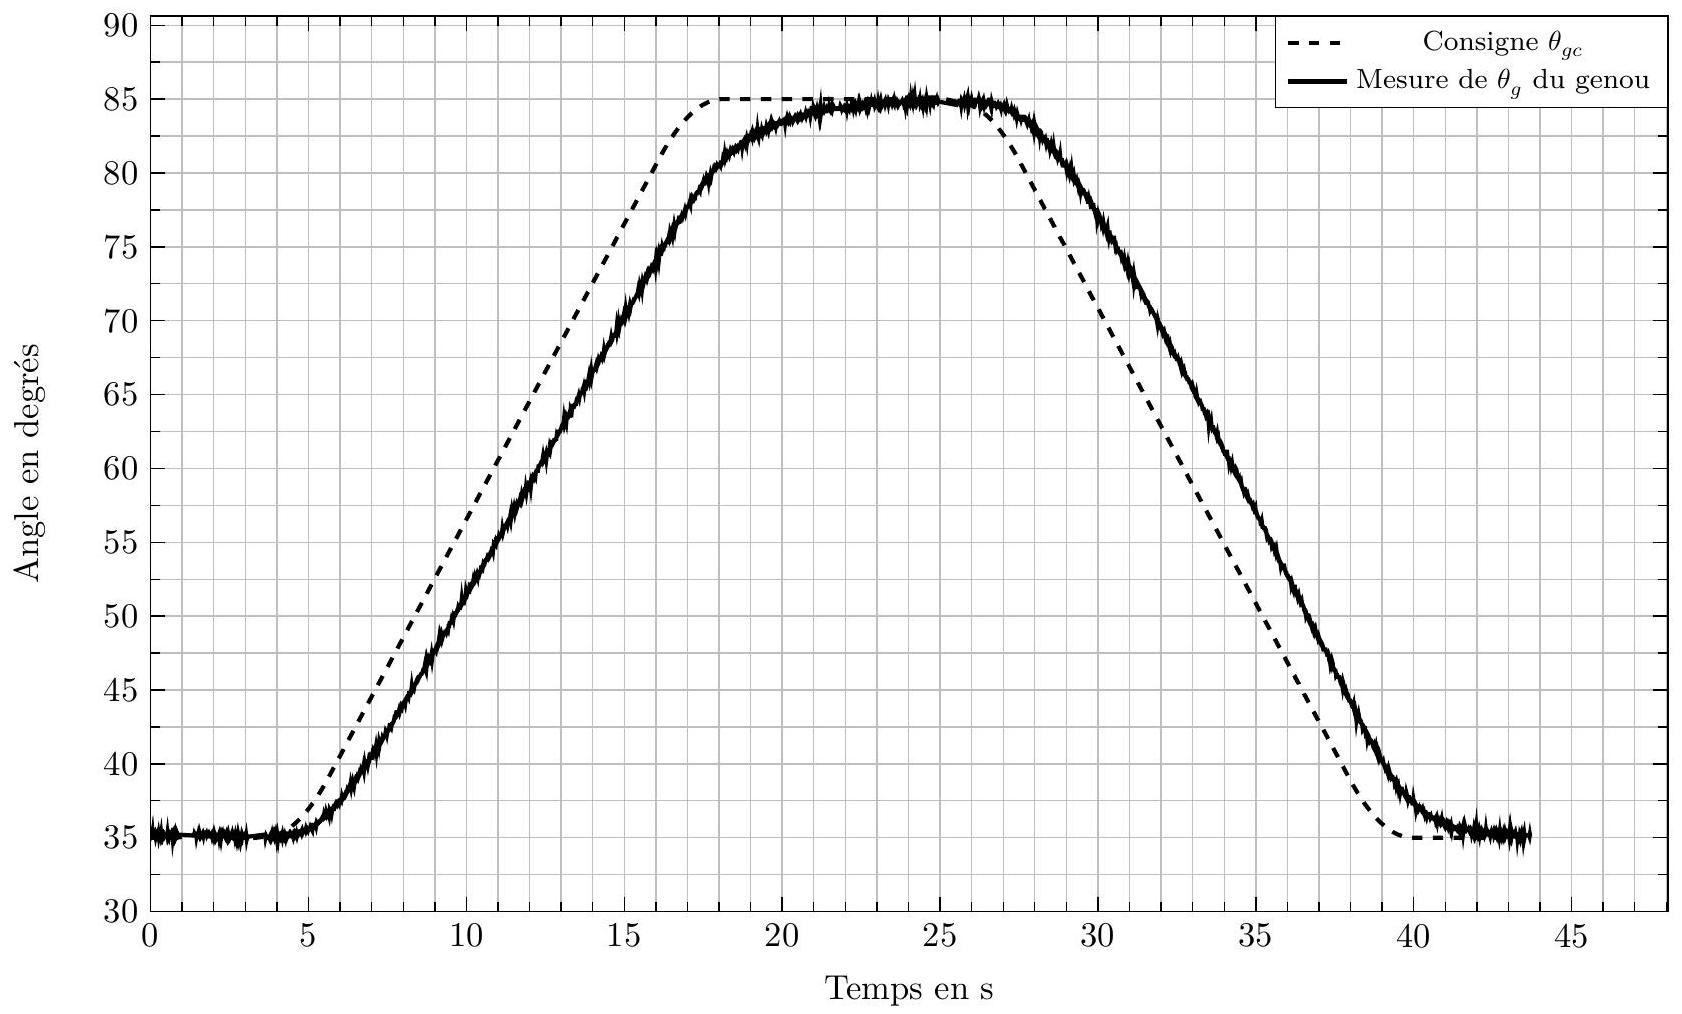
\includegraphics[max width=\textwidth]{2024_07_14_a83aebba33898893d39fg-04}
\caption{\label{fig:ccs_mp_2024:fig:06}Essai réalisé avec l'arthromoteur automatisé dont la carte de commande est paramétrée par défaut}
\end{figure}


%Q 2. 
\question{\label{q:ccs_mp_2024:02}En analysant les écarts avec les exigences 1.2.1 et 1.2.3, expliquer en quoi le réglage par défaut de la carte de commande de l'arthromoteur automatisé n'est pas acceptable. Argumenter avec des comparaisons quantifiées.}

\subsection{Problématique de l'étude}
Il apparait qu'en l'état, il est nécessaire de modifier les paramètres de la carte de commande de l'arthromoteur pour la rendre compatible avec les exigences de la rééducation.

\begin{obj}
L'objectif de l'étude est donc de déterminer les paramètres caractéristiques de la carte de commande angulaire du genou permettant à l'arthromoteur automatisé de générer un mouvement du genou conforme aux exigences de la rééducation.
\end{obj}
Pour répondre à la problématique, il faudra, dans un premier temps, établir un modèle de l'arthromoteur. Puis, à l'aide de ce modèle, il faudra déterminer les valeurs théoriques des paramètres de la carte de commande afin que le mouvement du genou soit conforme aux exigences. Les valeurs de réglage des paramètres seront implantées sur la carte de commande de l'arthromoteur et validées par un essai.

\section{Modélisation fonctionnelle de la structure de la commande angulaire du genou}
\begin{obj}
S'approprier l'environnement matériel en analysant la structure de la commande angulaire du genou de l'arthromoteur.
\end{obj}

Le thérapeute ou le patient fournit les informations nécessaires à l'élaboration de la consigne angulaire du genou $\indice{\theta}{g c}(t)$ à l'aide du pupitre de commande. Les exigences de la rééducation font apparaitre la nécessité de contrôler la position angulaire ainsi que la vitesse angulaire du genou. De plus, le mouvement demandé doit être suivi\\
sans être influencé par les caractéristiques morphologiques du patient, principalement les poids de la jambe et de la cuisse dans la cadre de la rééducation en mode passif. En conséquence, la structure de commande de la position du genou (figure \ref{fig:ccs_mp_2024:fig:07}) est basée sur une boucle d'asservissement en position angulaire du genou et un contrôle interne de vitesse.

\begin{figure}[!h]
\centering
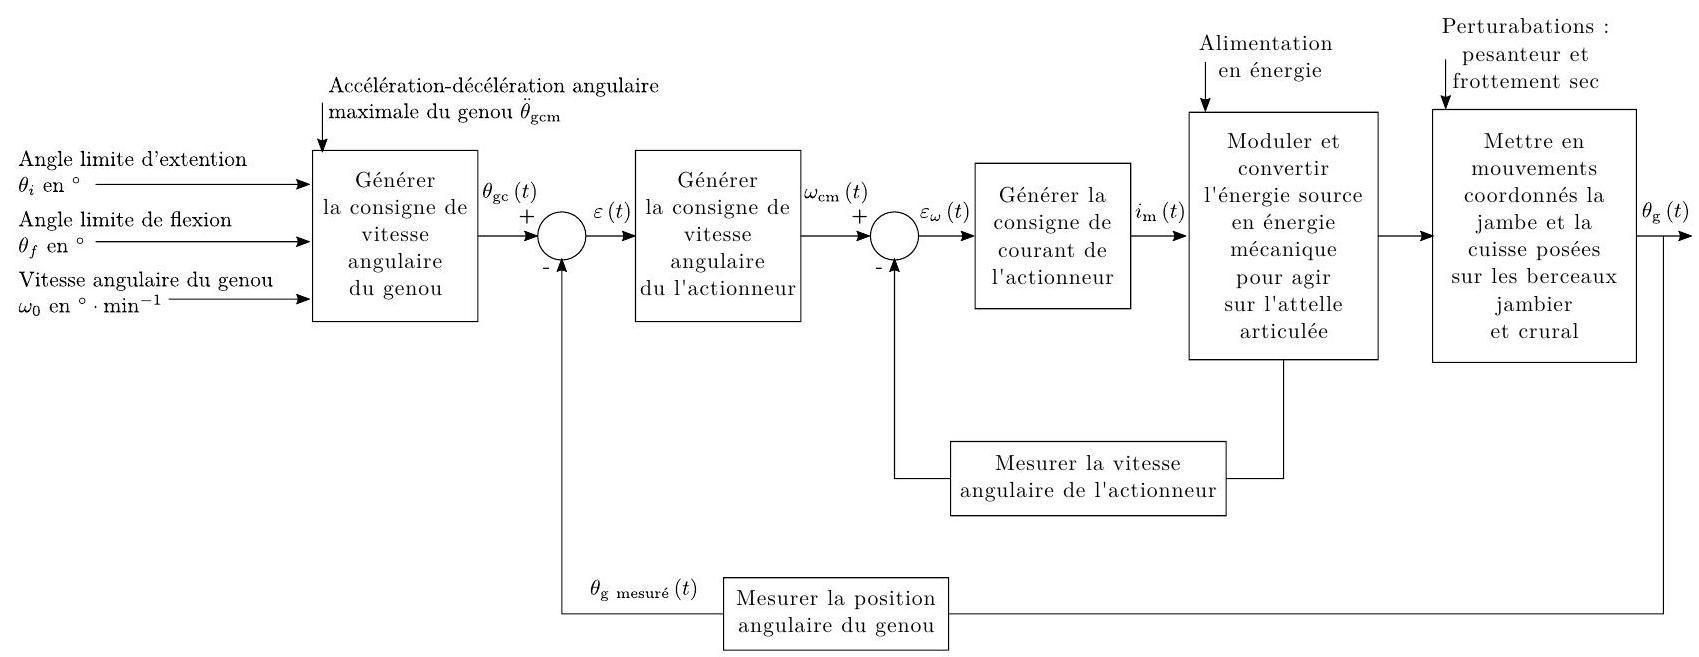
\includegraphics[max width=\textwidth]{2024_07_14_a83aebba33898893d39fg-05(1)}
\caption{\label{fig:ccs_mp_2024:fig:07}Structure de la commande en position angulaire du genou}
\end{figure}
Un capteur potentiométrique angulaire mesure la position angulaire du genou $\theta_{g}(t)$. L'écart $\varepsilon(t)=\theta_{g c}(t)-$ $\theta_{g \text { mesuré }}(t)$ est traité par la carte de commande pour générer la consigne de vitesse angulaire de l'actionneur électrique $\omega_{c m}(t)$. L'actionneur, piloté en courant, provoque le déplacement de la coulisse qui induit celui de l'attelle articulée sur laquelle sont posées la jambe et la cuisse. On appelle attelle articulée l'ensemble constitué du berceau crural, du berceau jambier, du bras et des deux biellettes, voir le diagramme BDD, figure \ref{fig:ccs_mp_2024:fig:32} en annexe.

%Q 3. 
\question{\label{q:ccs_mp_2024:03}À partir des éléments explicatifs sur le fonctionnement de l'arthromoteur et de son diagramme BDD (figure \ref{fig:ccs_mp_2024:fig:32}), identifier les constituants repérés de 1 à 6 ainsi que les flux 7 et 8 dans la description chaine d'information/chaine de puissance disponible en annexe (figure \ref{fig:ccs_mp_2024:fig:33}).}

La figure \ref{fig:ccs_mp_2024:fig:08} représente le schéma bloc fonctionnel simplifié de la structure de la commande angulaire du genou.

\begin{figure}[!h]\centering
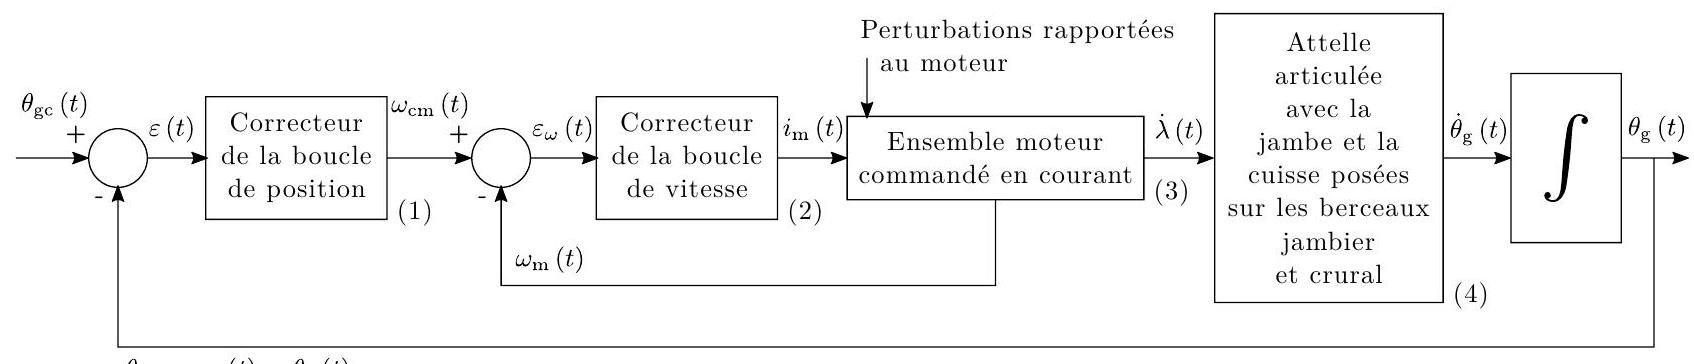
\includegraphics[max width=\textwidth]{2024_07_14_a83aebba33898893d39fg-05}

$\theta_{\mathrm{g} \text { mesuré }}(t)=\theta_{\mathrm{g}}(t)$

\caption{\label{fig:ccs_mp_2024:fig:08}Schéma bloc fonctionnel de la commande en position angulaire du genou}
\end{figure}

\subsection*{Notations et données :}
\begin{itemize}
  \item $\indice{\theta}{g c}(t)$ consigne angulaire du genou (en radians) ;

  \item $\theta_{g}(t)$ angle du genou (en radians) ;

  \item $\omega_{c m}(t)$ consigne de vitesse angulaire de l'axe moteur par rapport au bâti (en $\si{rad.s^{-1}}$ );

  \item $\omega_{m}(t)$ vitesse angulaire de l'axe moteur par rapport au bâti (en rad.s $\mathrm{s}^{-1}$ );

  \item $\lambda(t)$ déplacement de la coulisse 2 par rapport au bâti (en m) ;

  \item $i_{m}(t)$ intensité du moteur (en A).

\end{itemize}

Pour répondre à la problématique, il est nécessaire d'établir un modèle de l'arthromoteur (blocs (3) et (4) de la figure \ref{fig:ccs_mp_2024:fig:08}) et de déterminer les paramètres de la carte de commande (blocs (1) et (2) de la figure \ref{fig:ccs_mp_2024:fig:08}) en validant les choix théoriques effectués par des essais sur le matériel.

\section{Détermination des paramètres caractéristiques de la carte de commande angulaire du genou}
\begin{obj}
Établir un modèle de l'arthromoteur permettant de déterminer les valeurs théoriques des paramètres de la carte de commande garantissant que le mouvement du genou soit conforme aux exigences.
\end{obj}
\subsection{Modèle de connaissance linéaire de l'attelle articulée}

\begin{obj}
Déterminer un modèle linéaire du comportement cinématique de l'attelle articulée.
\end{obj}

\begin{figure}[!h]\centering
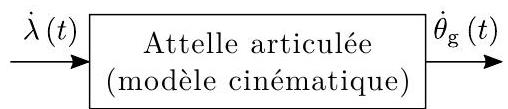
\includegraphics[width=.4\textwidth]{2024_07_14_a83aebba33898893d39fg-06}

\caption{\label{fig:ccs_mp_2024:fig:09}Entrée sortie du bloc fonctionnel modélisant l'attelle articulée}
\end{figure}
Le mécanisme est plan et de ce fait il ne sera considéré qu'une seule biellette. Le schéma cinématique plan de l'attelle articulée est fourni figure \ref{fig:ccs_mp_2024:fig:10}.

\begin{figure}[!h]\centering
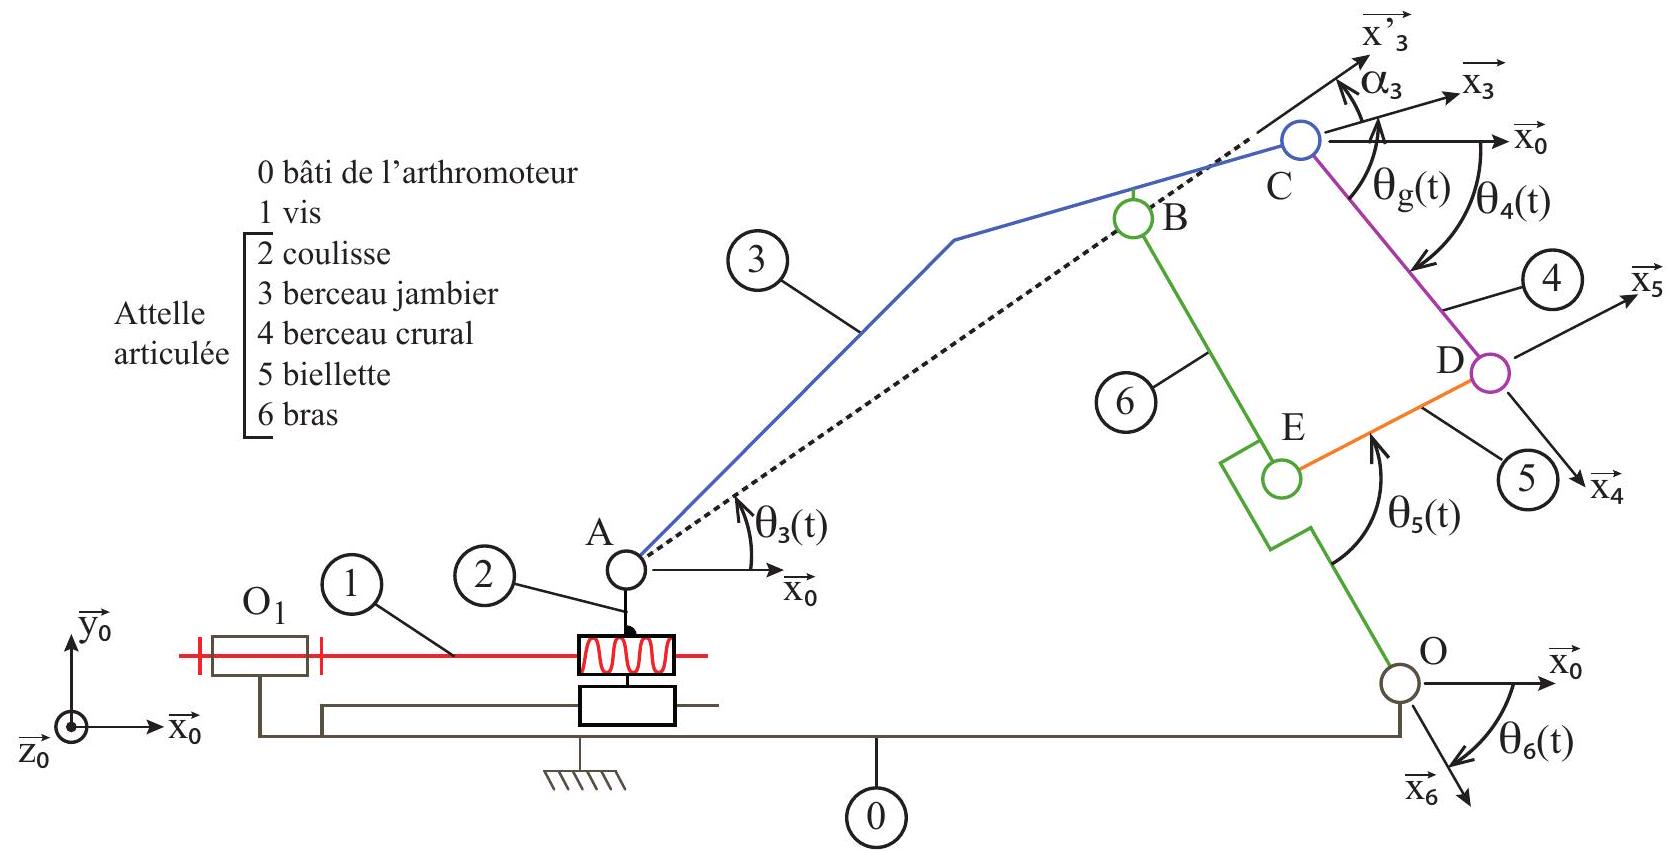
\includegraphics[max width=\textwidth]{2024_07_14_a83aebba33898893d39fg-06(1)}

\caption{\label{fig:ccs_mp_2024:fig:10}Schéma cinématique plan de l'arthromoteur}
\end{figure}

\subsubsection*{Paramétrage des solides }
\begin{itemize}
  \item le repère $R_{0}\left(O ; \vec{x}_{0}, \vec{y}_{0}, \vec{z}_{0}\right)$ est un repère galiléen lié au bâti 0 de l'arthromoteur avec $\overrightarrow{O_{1} O}=L_{0} \cdot \vec{x}_{0}-h \cdot \vec{y}_{0}$ ( $h$ et $L_{0}$ constants) ;
  \item les repères $R_{3}\left(A ; \vec{x}_{3}, \vec{y}_{3}, \vec{z}_{0}\right)$ et $R_{3}^{\prime}\left(C ; \vec{x}_{3}, \vec{y}_{3}, \vec{z}_{0}\right)$ sont liés au berceau jambier 3 avec $\alpha_{3}=\left(\vec{x}_{3}, \vec{x}_{3}\right)\left(\alpha_{3}\right.$ constant) et $\overrightarrow{A B}=L_{3} \cdot \overrightarrow{x^{\prime}}{ }_{3}$ ( $L_{3}$ constant);
  \item le repère $R_{4}\left(C ; \vec{x}_{4}, \vec{y}_{4}, \vec{z}_{0}\right)$ est lié au berceau crural 4;
  \item le repère $R_{5}\left(E ; \vec{x}_{5}, \vec{y}_{5}, \vec{z}_{0}\right)$ est lié à la biellette 5 ;
  \item le repère $R_{6}\left(O ; \vec{x}_{6}, \vec{y}_{6}, \vec{z}_{0}\right)$ est lié au bras 6 avec $\overrightarrow{B O}=L_{6} \cdot \vec{x}_{6}$ ( $L_{6}$ constant).
\end{itemize}
\subsection*{Paramétrage des liaisons :}
\begin{itemize}
  \item pour la liaison 0-1 et la liaison 1-2, $\overrightarrow{O_{1} A}=\lambda(t) \cdot \vec{x}_{0}+h_{0} \vec{y}_{0}$;
  \item pour la liaison 2-3, $\theta_{3}(t)=\left(\vec{x}_{0}, \vec{x}_{3}\right)=\left(\vec{y}_{0}, \vec{y}_{3}\right)$;
  \item pour la liaison 3-4, $\theta_{g}(t)=\left(\vec{x}_{4}, \vec{x}_{3}\right)=\left(\vec{y}_{4}, \vec{y}_{3}\right)$ angle du genou et $\theta_{4}(t)=\left(\vec{x}_{0}, \vec{x}_{4}\right)=\left(\vec{y}_{0}, \vec{y}_{4}\right)$;
  \item pour la liaison 5-6, $\theta_{5}(t)=\left(\vec{x}_{6}, \vec{x}_{5}\right)=\left(\vec{y}_{6}, \vec{y}_{5}\right)$;
  \item pour la liaison 0-6, $\theta_{6}(t)=\left(\vec{x}_{0}, \vec{x}_{6}\right)=\left(\vec{y}_{0}, \vec{y}_{6}\right)$.
\end{itemize}

%Q 4. 
\question{\label{q:ccs_mp_2024:04}Donner l'expression de l'angle du genou $\theta_{g}(t)$ en fonction des angles $\theta_{3}(t), \theta_{4}(t)$ et $\alpha_{3}$.}

%Q 5. 
\question{\label{q:ccs_mp_2024:05}En exploitant la relation de fermeture géométrique de la chaine fermée de liaisons et de solides \{0-1-2-3-6-0\}, déterminer l'expression de $\lambda(t)$ en fonction de l'angle $\theta_{3}(t)$ et des paramètres géométriques constants $L_{0}, L_{3}, L_{6}, h$ et $h_{0}$.}

Grâce aux questions Q. \ref{q:ccs_mp_2024:04} et Q. \ref{q:ccs_mp_2024:05} et en exploitant une autre chaine de solides fournissant l'expression de $\theta_{4}(t)$ en fonction de $\theta_{3}(t)$ (non abordée dans ce sujet), il est possible d'avoir l'expression de $\theta_{g}(t)$ en fonction de $\lambda(t)$. La figure \ref{fig:ccs_mp_2024:fig:11} représente le tracé de l'angle $\theta_{g}(t)$ en fonction du déplacement $\lambda(t)$ de la coulisse 2 pour un mouvement angulaire du genou de $35^{\circ}$ à $85^{\circ}$. Le tracé montre un comportement quasi linéaire dans la zone angulaire fonctionnelle pour la rééducation des ligaments croisés. Il est décidé de procéder à une régression linéaire afin d'obtenir la loi entrée-sortie géométrique de l'attelle articulée : $\theta_{g}(t)=f(\lambda(t))$.

\begin{figure}[!h]\centering
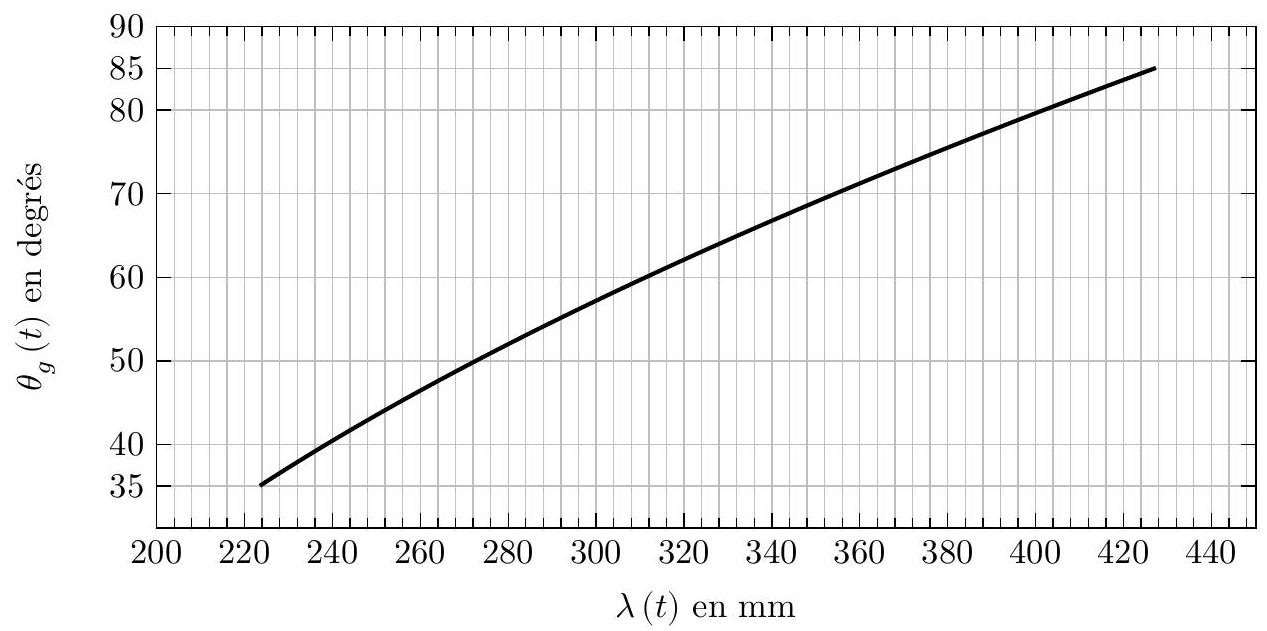
\includegraphics[max width=\textwidth]{2024_07_14_a83aebba33898893d39fg-07}

\caption{\label{fig:ccs_mp_2024:fig:11}Angle du genou $\theta_{g}(t)$ en fonction du déplacement $\lambda(t)$ de la coulisse 2}
\end{figure}

La régression linéaire consiste à chercher les paramètres $a$ et $b$ définissant la droite $\theta_{g}(t)=a \cdot \lambda(t)+b$ et qui passe au plus près de l'ensemble des points $\left(\lambda_{k}, \theta_{g k}\right)$. Les points $\left(\lambda_{k}, \theta_{g k}\right)$ sont obtenus en faisant varier $\lambda(t)$ et en calculant les différentes valeurs $\theta_{g k}$ correspondantes grâce à la loi entrée-sortie $\theta_{g}(t)=f(\lambda(t))$ déterminée à partir des questions précédentes.

Les paramètres $a$ et $b$ sont à déterminer par la méthode des moindres carrés qui consiste ici à minimiser la fonction cout $Q(a, b)$ pour les n points $\left(\lambda_{k_{k \in[1, n]}}, \theta_{g k_{k \in[1, n]}}\right)$ connus, avec $Q(a, b)=\sum_{k=1}^{n}\left(\theta_{g k}-a \cdot \lambda_{k}-b\right)^{2}$.

%Q 6.
\question{\label{q:ccs_mp_2024:06}Donner le système de deux équations liant $\theta_{g k_{k \in[1, n]}}, \lambda_{k_{k \in[1, n]}}, a$ et $b$ et traduisant le fait que $a$ et $b$ minimisent $Q(a, b)$.}

%Q 7. 
\question{\label{q:ccs_mp_2024:07}Donner les expressions de $a$ et de $b$ solutions du système d'équations défini précédemment. $a$ et $b$ sont fonction de $n$, de $\theta_{g k_{k \in[1, n]}}$ et de $\lambda_{k_{k \in[1, n]}}$.}

Pour obtenir l'expression linéaire de $\theta_{g}(t)$ en fonction de $\lambda(t)$, la régression linéaire est mise en oeuvre en langage Python. Les données disponibles sont les listes $T$ et $L$ composées respectivement des valeurs $\theta_{g k}$ et $\lambda_{k}$ issues du script python qui a permis d'obtenir la figure \ref{fig:ccs_mp_2024:fig:11}. Les listes $L$ et $T$ sont de même longueur.

%Q 8. 
\question{\label{q:ccs_mp_2024:08}Écrire en langage Python une fonction $S u m_{-} L i(L i)$ qui prend en argument une liste $L i$ de nombres à virgule flottante et qui renvoie la somme des termes de cette liste.
Écrire en langage Python une fonction \lstinline{Sum_Li_2(Li)} qui prend en argument une liste $L i$ de nombres à virgule flottante et qui renvoie la somme des termes au carré de cette liste.
Écrire une fonction \lstinline{Sum_XY(X,Y)} qui prend en argument deux listes $X$ et $Y$ de nombres à virgule flottante, de même longueur et qui renvoie la somme des produits $x_{k} \cdot y_{k}$ avec $x_{k}$ et $y_{k}$ les termes des listes $X$ et $Y$.}

\question{\label{q:ccs_mp_2024:09}Écrire en langage Python une fonction $\operatorname{reg} \operatorname{lin}(L, T)$ prenant en argument les listes $L$ et $T$ retournant les valeurs de $a$ et de $b$ définissant la relation $\theta_{g}(t)=a \cdot \lambda(t)+b$.}

La mise en oeuvre de la fonction reg\_lin permet d'obtenir $a=4,25$ en $\left(\mathrm{rad} \cdot \mathrm{m}^{-1}\right)$ et donc d'écrire la loi entréesortie de l'attelle articulée d'un point de vue cinématique, puisque $\dot{\theta}_{g}(t)=a \cdot \dot{\lambda}(t)$.

En procédant avec la même démarche pour les angles $\theta_{3}$ et $\theta_{4}$, il est possible d'obtenir : $\dot{\theta}_{3}(t)=K_{3} \cdot \dot{\theta}_{g}(t)$ et $\dot{\theta}_{4}(t)=K_{4} \cdot \dot{\theta}_{g}(t)$. Par la suite $\dot{\theta}_{g}(t)=a \cdot \dot{\lambda}(t), \dot{\theta}_{3}(t)=K_{3} \cdot \dot{\theta}_{g}(t)$ et $\dot{\theta}_{4}(t)=K_{4} \cdot \dot{\theta}_{g}(t)$ avec $a=\SI{4,25}{rad.m^{-1}}$, $K_{3}=0,34$ (sans unité) et $K_{4}=-0,66$ (sans unité).

Le modèle cinématique linéaire de l'attelle articulée étant maintenant établi, l'étude va se poursuivre avec la modélisation, l'identification et le réglage de la vitesse angulaire de l'ensemble moteur.

\subsection{Modélisation, identification et réglage de la boucle de vitesse}
\begin{obj}
Déterminer et valider un modèle de la commande en vitesse angulaire du moteur de l'arthromoteur.
\end{obj}

La figure \ref{fig:ccs_mp_2024:fig:12} représente le schéma bloc fonctionnel de la commande en vitesse de l'ensemble moteur.

\begin{figure}[!h]\centering
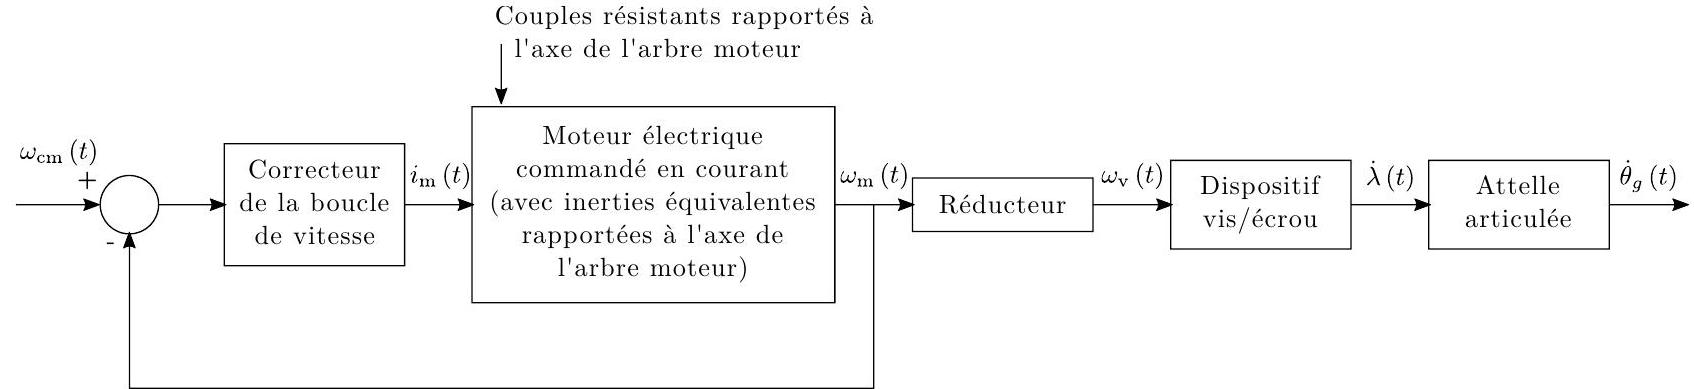
\includegraphics[max width=\textwidth]{2024_07_14_a83aebba33898893d39fg-08}
\caption{\label{fig:ccs_mp_2024:fig:12}Schéma bloc fonctionnel de la commande en vitesse angulaire du genou}
\end{figure}
\subsubsection*{Notations}
\begin{itemize}
  \item $\omega_{v}(t)$ vitesse angulaire de la vis 1 par rapport au bâti (en rad.s ${ }^{-1}$ );

  \item $i_{m}(t)$ intensité du moteur (en A) ;

  \item le couple exercé par le stator sur le rotor du moteur est noté $C_{m}(t)$ avec $C_{m}(t)=k_{t} \cdot i_{m}(t)$ et $k_{t}=0,0256 \mathrm{~N} \cdot \mathrm{m} \cdot \mathrm{A}^{-1}$.

\end{itemize}

\subsubsection{Modèle de comportement dynamique de la boucle de vitesse de l'arthromoteur automatisé}
 \subsubsection*{Données et hypothèses}
\begin{itemize}
  \item Cinétique :
\begin{itemize}
  \item le moment d'inertie équivalent de l'ensemble \{arbre moteur, réducteur, vis (1)\} rapporté à l'axe de l'arbre moteur $\left(O_{1}, \vec{x}_{0}\right)$ est noté $J_{\text {eqmot }}$;
  \item la masse équivalente maximale en translation des solides constituants l'attelle, y compris la jambe posée sur le berceau jambier et la cuisse posée sur le berceau crural, rapportée à la direction du mouvement de la coulisse $2 \vec{x}_{0}$, est notée $m_{2}$ avec $m_{2}<0,49 \mathrm{~kg}$;
\end{itemize}
  \item Actions mécaniques :
\begin{itemize}
  \item les liaisons mécaniques entre les solides en mouvement et le bâti sont supposées parfaites ;
  \item le couple équivalent de pesanteur rapporté à l'axe de l'arbre moteur est noté $C_{\text {pes }}$, ce couple peut être considéré comme étant dû à la présence de la cuisse et de la jambe sur l'attelle (la masse de l'ensemble jambe+cuisse est en moyenne 10 fois supérieure à celle de la masse totale des berceaux) ;
  \item du fait de leur structure et de leur matériau, les masses des berceaux sont suffisamment faibles pour négliger l'action mécanique de pesanteur sur les composants de l'attelle articulée ;
  \item le couple équivalent de frottement visqueux dans l'ensemble du système et rapporté à l'axe de l'arbre moteur a pour expression $C_{f}(t)=-f_{v} \cdot \omega_{m}(t)$;
  \item le couple équivalent de frottement sec dans l'ensemble du système et rapporté à l'axe de l'arbre moteur est noté $C_{\text {sec }}=-\operatorname{signe}\left(\omega_{m}(t)\right) \cdot K_{\mathrm{sec}}$ avec $K_{\mathrm{sec}}>0$;
\end{itemize}
\item Cinématique :
\begin{itemize}
  \item le réducteur a un rapport de réduction $K_{r}=\frac{\omega_{v}(t)}{\omega_{m}(t)}=\frac{1}{16}$;
  \item le dispositif vis/écrou est modélisable par un gain $K_{v}=\frac{\dot{\lambda}(t)}{\omega_{v}(t)}=\frac{5 \cdot 10^{-3}}{2 \pi}$ exprimé en m.rad ${ }^{-1}$.
\end{itemize}
\end{itemize}

L'application du théorème de l'énergie cinétique à l'ensemble $\Sigma=$ arbre moteur, réducteur, 1, 2, 3, 4, 5, 6 , jambe, cuisse\} permet d'écrire :

$$
J_{\mathrm{eq}} \cdot \frac{\dd \omega_{m}(t)}{\dd t}=C_{m}(t)-f_{v} \cdot \omega_{m}(t)+C_{\mathrm{sec}}+C_{\mathrm{pes}} %\tag{III.1}
$$

$J_{\text {eq }}$ est le moment d'inertie équivalente de l'ensemble $\Sigma$ rapportée à l'arbre moteur.

%Q 10. 
\question{\label{q:ccs_mp_2024:10}Réaliser l'inventaire des puissances des actions mécaniques extérieures et intérieures à l'ensemble $\Sigma$ qui a permis d'obtenir l'équation (1). L' expression des puissances est demandée et les justifications apportées doivent être claires et précises. L'inventaire doit être réalisé soigneusement de manière à distinguer nettement les puissances extérieures et intérieures.}

\subsubsection{Identification des grandeurs caractéristiques de l'ensemble moteur}

\begin{obj}
Déterminer un modèle de l'ensemble moteur et identifier ses constantes en l'absence de la cuisse et de la jambe dans un premier temps.
\end{obj}

\paragraph*{Premier essai en l'absence de la cuisse et de la jambe}
Pour déterminer le coefficient de frottement visqueux $f_{v}$ et le couple de frottement sec $C_{\text {sec }}$, des essais en flexion sont réalisés sur l'arthromoteur sans le patient.

\paragraph*{— Conditions matérielles $\mathrm{N}^{\circ} 1$}
Pendant ces essais, la boucle d'asservissement en angle est désactivée pour ne garder que l'asservissement en vitesse du moteur.

\paragraph*{— Protocole de mesure $\mathrm{N}^{\circ} 1$}
Plusieurs consignes de vitesse $\omega_{c m}(t)$ de type échelon sont envoyées en entrée de la carte de commande.

L'intensité $i_{m}(t)$ du moteur ainsi que sa vitesse de rotation $\omega_{m}(t)$ sont mesurées en régime permanent.

Les conditions de mise en œuvre de ce premier essai sont résumées sur la figure \ref{fig:ccs_mp_2024:fig:13}.

\begin{figure}[!h]\centering
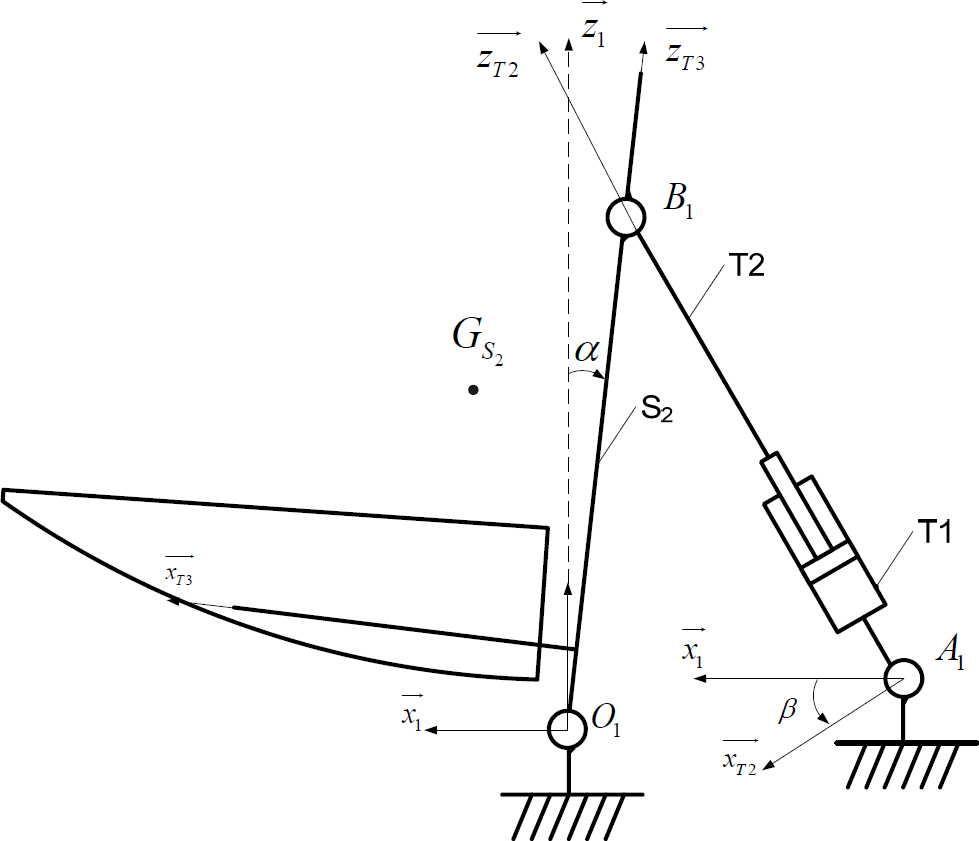
\includegraphics[max width=.6\textwidth]{fig_13}

\caption{\label{fig:ccs_mp_2024:fig:13}Résumé des conditions de mise en œuvre du premier essai}
\end{figure}
La figure \ref{fig:ccs_mp_2024:fig:14} représente le relevé expérimental fournissant les mesures de l'intensité moteur en régime permanent $i_{m}$ en fonction de la vitesse de rotation du moteur en régime permanent $\omega_{m}$.

%Q 11. 
\question{\label{q:ccs_mp_2024:11}Écrire l'équation (1) en régime permanent dans les conditions matérielles $\mathrm{N}^{\circ} 1$ et déduire de la figure \ref{fig:ccs_mp_2024:fig:14} la valeur numérique du coefficient de frottement visqueux $f_{v}$ et du couple de frottement $\sec C_{\mathrm{sec}}$.}

\begin{figure}[!h]\centering
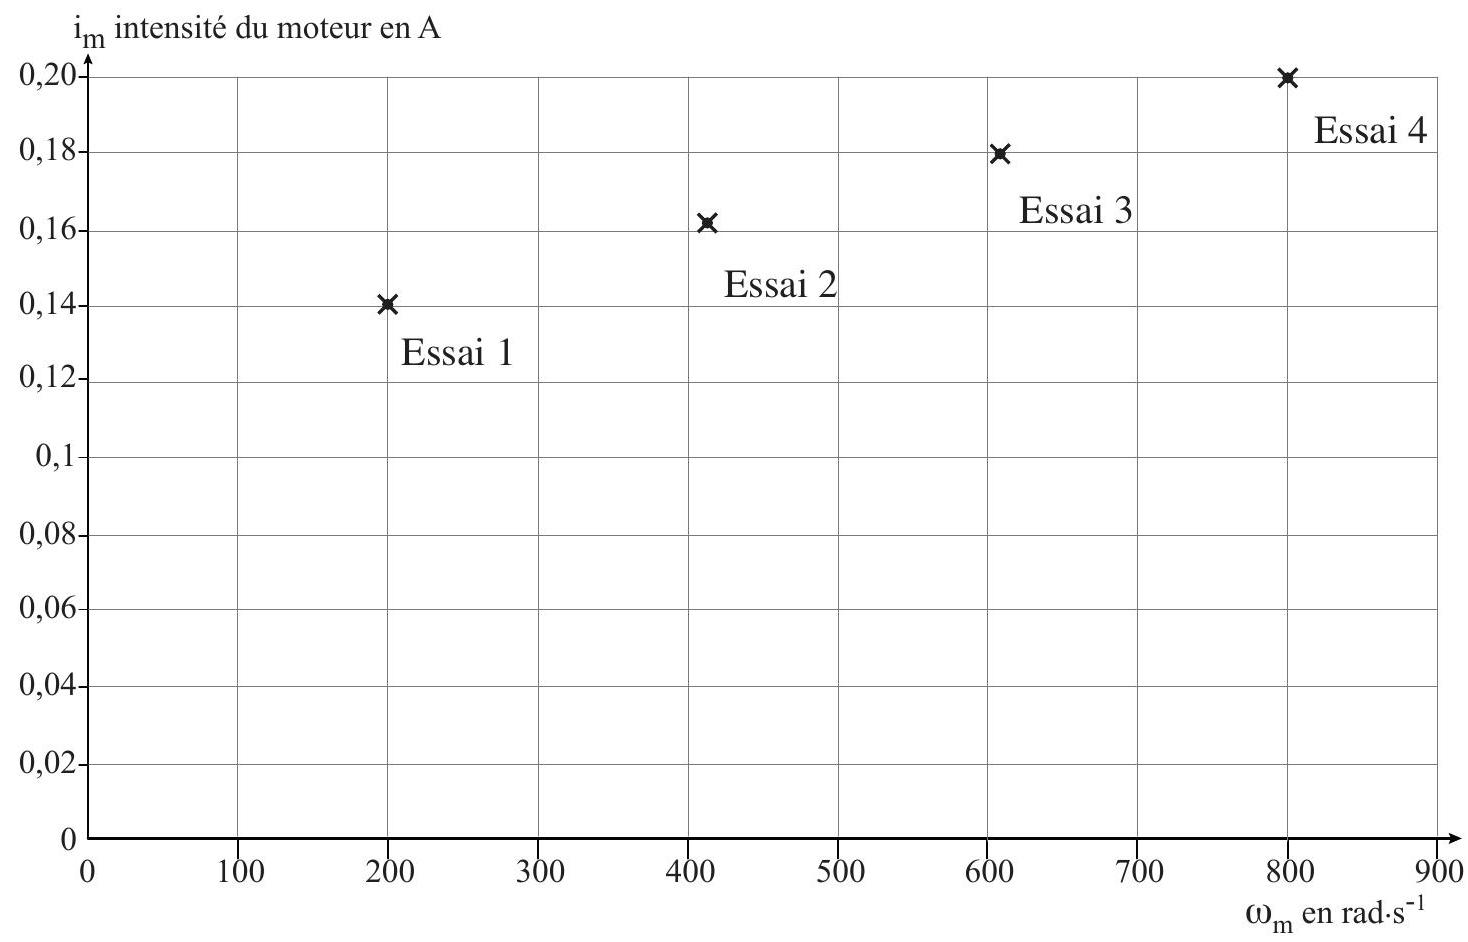
\includegraphics[max width=.7\textwidth]{2024_07_14_a83aebba33898893d39fg-09(1)}
\caption{\label{fig:ccs_mp_2024:fig:14}Intensité $i_{m}$ en fonction de $\omega_{m}$ en régime permanent}
\end{figure}
\paragraph*{Deuxième essai en l'absence de la cuisse, de la jambe et de l'attelle articulée}

\paragraph*{— Conditions matérielles $\mathrm{N}^{\circ} 2$}
Pour déterminer l'inertie équivalente $J_{\text {eqmot }}$ de la motorisation de l'arthromoteur, un essai (figure \ref{fig:ccs_mp_2024:fig:17}) a été réalisé avec la liaison pivot entre la coulisse 2 et le berceau jambier 3 démontée pour ne pas prendre en compte l'effet du frottement sec principalement présent dans l'attelle articulée. Ainsi, l'attelle articulée n'est pas mise en mouvement. Dans cette configuration de l'essai, il est possible de faire l'hypothèse qu'il n'y a pas de frottement sec.

La structure de commande pour réaliser l'essai est représenté figure \ref{fig:ccs_mp_2024:fig:15}. Cette structure correspond à celle utilisée dans l'arthromoteur pour asservir le moteur en vitesse. Après avoir transformé les équations temporelles dans le domaine de Laplace, on peut représenter la boucle de vitesse comme sur la figure \ref{fig:ccs_mp_2024:fig:15}.

\begin{figure}[!h]\centering
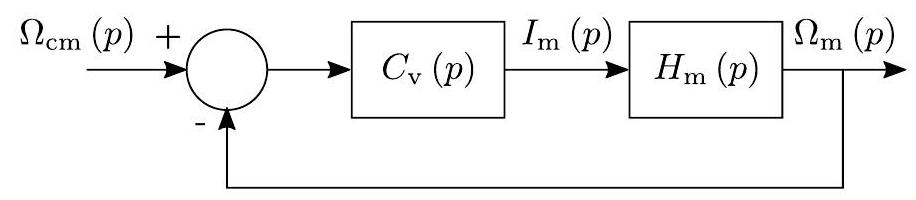
\includegraphics[max width=.5\textwidth]{2024_07_14_a83aebba33898893d39fg-10}
\caption{\label{fig:ccs_mp_2024:fig:15}Commande utilisée pour l'essai en consigne de vitesse du moteur}
\end{figure}

%Q 12.
\question{\label{q:ccs_mp_2024:12}En considérant les conditions initiales nulles, déterminer l'expression de la fonction de transfert du moteur $H_{m}(p)=\frac{\Omega_{m}(p)}{I_{m}(p)}$ de l'asservissement en vitesse du moteur.}

La carte de commande comporte un correcteur de fonction de transfert $C_{v}(p)$ qui est de type proportionnel pour l'essai réalisé : $C_{v}(p)=K_{p}$ avec $K_{p}=0,0094 \mathrm{~A} \cdot \mathrm{s} \cdot \mathrm{rad}^{-1}$ (valeur par défaut implantée dans la carte de commande).

\paragraph*{— Protocole de mesure N°2}
Une mesure de la vitesse angulaire du moteur $\omega_{m}(t)$ est réalisée pour une consigne en échelon de vitesse $\omega_{c m}(t)=\omega_{m 0}$ avec $\omega_{m 0}=285 \si{rad.s^{-1}}$.

Les conditions de mise en œuvre du deuxième essai sont résumées figure \ref{fig:ccs_mp_2024:fig:16}.

\begin{figure}[!h]\centering
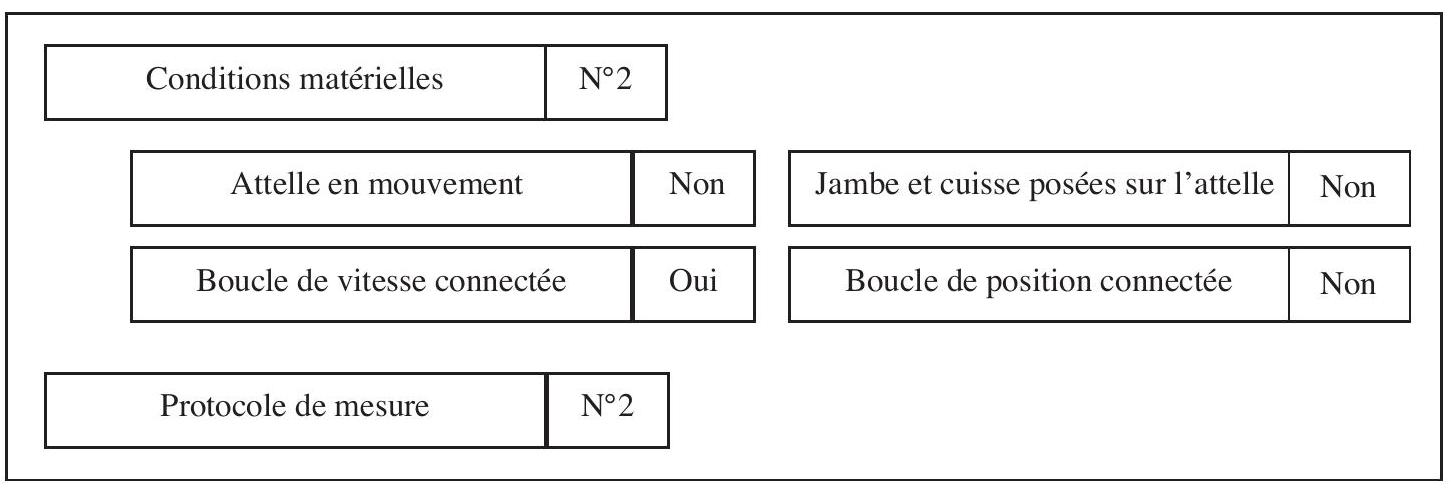
\includegraphics[max width=.7\textwidth]{2024_07_14_a83aebba33898893d39fg-10(1)}
\caption{\label{fig:ccs_mp_2024:fig:16}Résumé des conditions de mise en œuvre du deuxième essai}
\end{figure}
La figure \ref{fig:ccs_mp_2024:fig:17} est le résultat de ce deuxième essai.

%Q 13. 
\question{\label{q:ccs_mp_2024:13}Donner l'expression littérale sous forme canonique de la fonction de transfert $H_{v}(p)=\frac{\Omega_{m}(p)}{\Omega_{c m}(p)}$ en fonction de $K_{p}, J_{\text {eqmot }}, k_{t}$ et $f_{v}$.}

%Q 14. 
\question{\label{q:ccs_mp_2024:14}Déduire de l'essai figure \ref{fig:ccs_mp_2024:fig:17} la valeur numérique de l'inertie équivalente $J_{\text {eqmot }}$.}

%Q 15. 
\question{\label{q:ccs_mp_2024:15}Déterminer l'expression de $J_{\text {eq }}$ en fonction de $J_{\text {eqmot }}, m_{2}, K_{v}$ et $K_{r}$. Montrer que $J_{\text {eq }} \approx J_{\text {eqmot }}$.}

\paragraph*{Validation des hypothèses}
Le couple équivalent de frottement sec rapporté à l'axe de l'arbre moteur peut provenir de l'attelle articulée ou de l'ensemble moteur, soit : $C_{\mathrm{sec}}=C_{\text {sec.moteur }}+C_{\text {sec.attelle }}$. De même pour le frottement visqueux qui peut s'écrire $f_{v}=f_{\text {v.moteur }}+f_{\text {v.attelle }}$.

Lors du second essai, l'hypothèse de l'absence de frottement sec, en l'absence de l'attelle, implique que

$C_{\text {sec.moteur }} \approx 0$. La valeur de $f_{v}$, déterminée avec le premier essai, a été utilisée pour exploiter la mesure du deuxième essai, ce qui implique que l'hypothèse $f_{\text {v.attelle }} \approx 0$ a été implicitement faite.

%Q 16.
\question{\label{q:ccs_mp_2024:16}Proposer les conditions matérielles $\left(\mathrm{N}^{\circ} 1\right.$ ou $\left.\mathrm{N}^{\circ} 2\right)$ ainsi que le protocole de mesure $\left(\mathrm{N}^{\circ} 1\right.$ ou $\left.\mathrm{N}^{\circ} 2\right)$ d'un troisième essai qui valideraient les hypothèses $C_{\text {sec.moteur }} \approx 0$ et $f_{\text {v.attelle }} \approx 0$. Justifier brièvement ce choix, reproduire la figure \ref{fig:ccs_mp_2024:fig:18} sur la copie puis compléter pour résumer les conditions de mise en œuvre de l'essai retenu.}

Le modèle de l'ensemble moteur de l'arthromoteur est maintenant établi. Il reste à évaluer l'influence de l'action de pesanteur de la jambe et de la cuisse du patient afin de compléter ce modèle.

\begin{figure}[!h]\centering
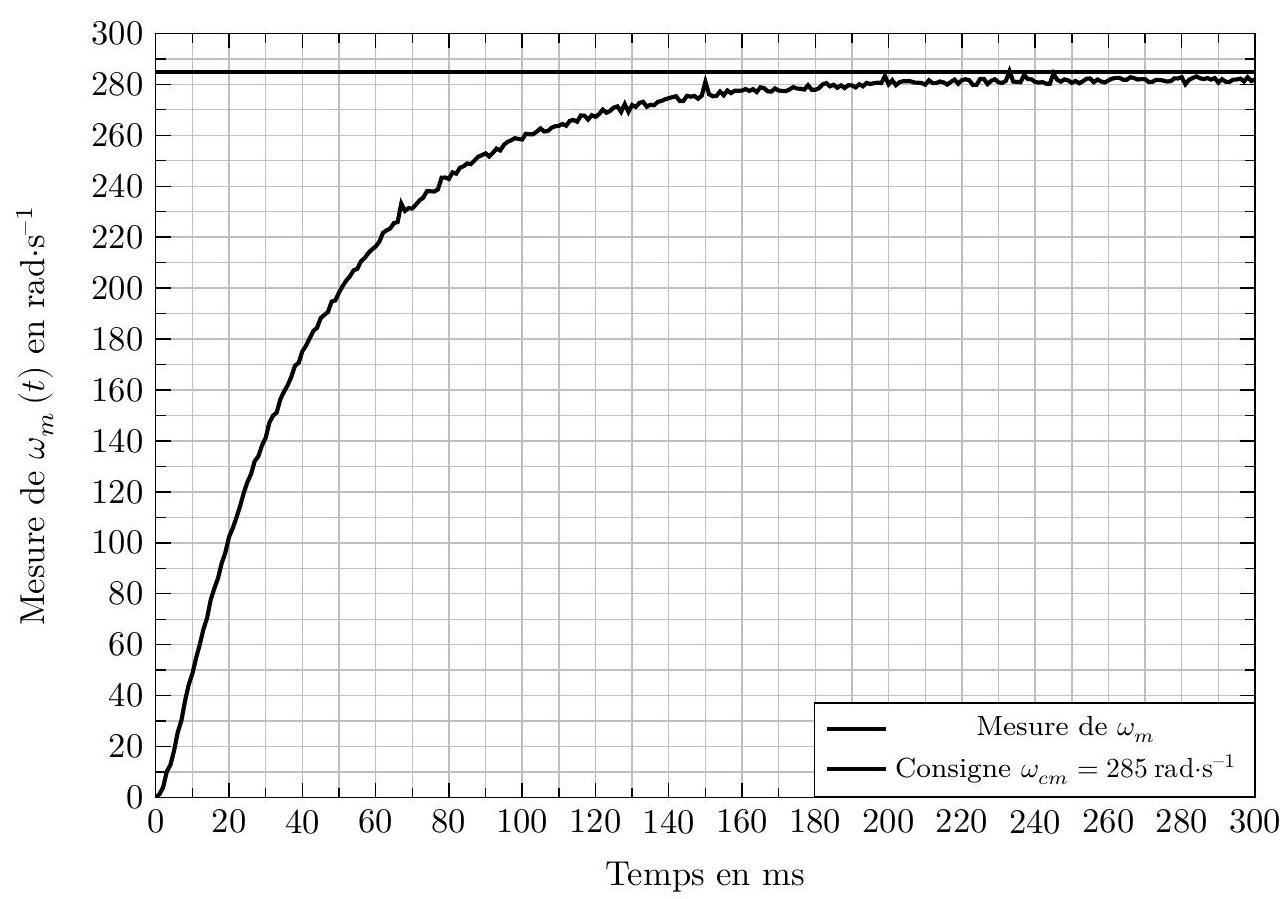
\includegraphics[max width=.7\textwidth]{2024_07_14_a83aebba33898893d39fg-11(1)}

\caption{\label{fig:ccs_mp_2024:fig:17}Vitesse de rotation du moteur pour une consigne en échelon de vitesse de $285 \si{rad.s^{-1}}$}
\end{figure}


\begin{figure}[!h]\centering
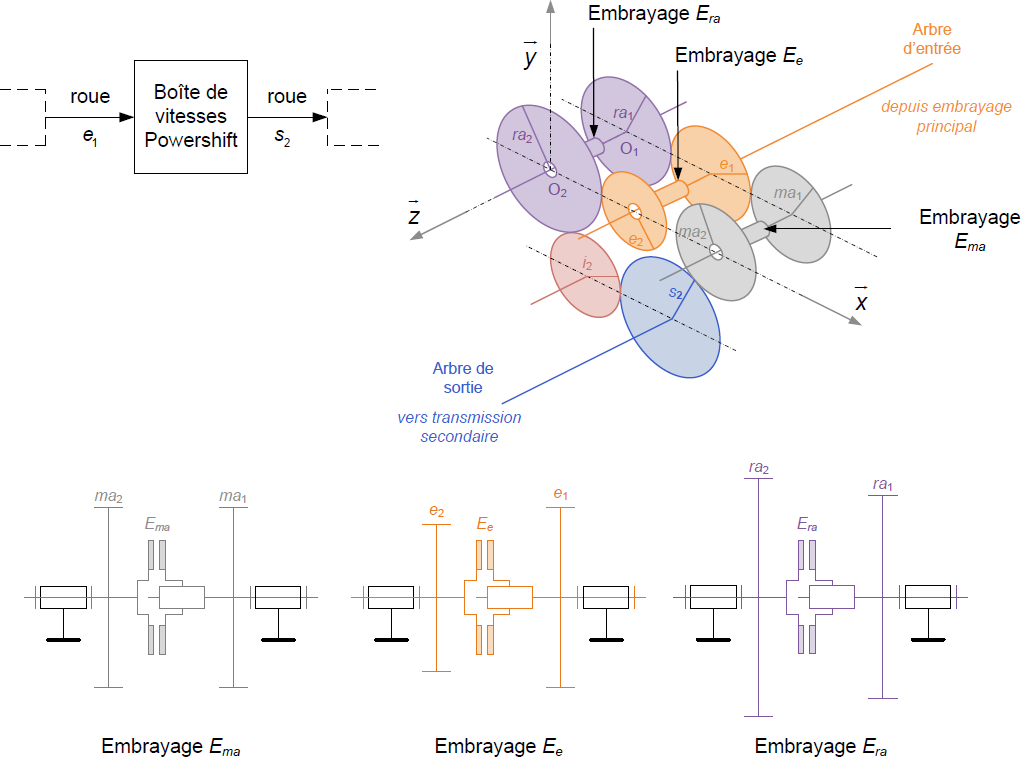
\includegraphics[max width=\textwidth]{fig_18}

\caption{\label{fig:ccs_mp_2024:fig:18}Résumé des conditions de mise en œuvre
d'un essai de validation de $C_{\text {sec.moteur }} \approx 0$ et $f_{\text {v.attelle }} \approx 0$}
\end{figure}




\subsubsection{Détermination des grandeurs caractéristiques du couple résistant dû à l'action de pesanteur}
\begin{obj}
Évaluer le couple équivalent rapporté à l'axe moteur dû à l'action de pesanteur exercée sur la jambe et la cuisse puis compléter le modèle de l'ensemble moteur en conséquence.
\end{obj}
L'action de la pesanteur qui s'exerce sur la jambe et la cuisse est modélisée par un couple équivalent rapporté à l'arbre moteur noté $C_{\text {pes }}$.

La figure \ref{fig:ccs_mp_2024:fig:19} représente le système avec la jambe et la cuisse du patient positionnées sur l'attelle articulée. La figure \ref{fig:ccs_mp_2024:fig:20} fournit le paramétrage relatif à la jambe et la cuisse.

\subsection*{Hypothèses}
\begin{itemize}
  \item le centre de l'articulation cuisse/hanche est noté $C_{h}$ et est supposé fixe dans le repère $R_{0}$ lié au bâti de l'arthromoteur ;

  \item la structure des berceaux est telle que le centre $C_{g}$ du genou du patient est confondu avec le centre $C$ de la liaison pivot $3 / 4$;

  \item la cuisse et le berceau crural sont en mouvement de rotation autour de l'axe de la hanche $\left(C_{h}, \vec{z}_{0}\right)$;

\end{itemize}

\subsection*{Notations et données }
\begin{itemize}
 \item on note $\vec{g}=-g \cdot \vec{y}_{0}$ l'accélération de la pesanteur ;
 \item  le solide 3 correspond à l'ensemble \{berceau jambier + jambe $\}$ et le solide 4 à $\{$ berceau crural + cuisse $\}$;
  \item $\indice{L}{cu}$ longueur de la cuisse ;
 \item les points $C_{h}$ et $C_{g}$ correspondent respectivement au centre de l'articulation hanche/cuisse et au centre de l'articulation cuisse/jambe (centre du genou) ;
  \item le point $G_{c}$ est le centre de gravité de la cuisse et $G_{j}$ celui de la jambe ;
  \item $\overrightarrow{G_{j} C}=L_{j} \cdot \vec{x}_{3}, \overrightarrow{C C_{h}}=\indice{L}{cu} \cdot \vec{x}_{4}$ (données anatomiques disponibles figure \ref{fig:ccs_mp_2024:fig:20}). 
\end{itemize}

\begin{figure}[!h]\centering
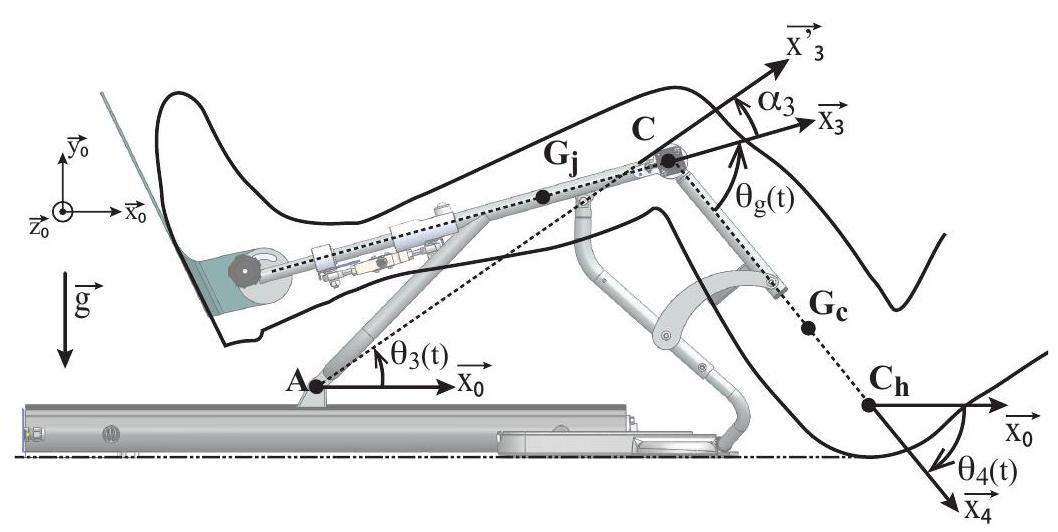
\includegraphics[max width=\textwidth]{2024_07_14_a83aebba33898893d39fg-12}

\caption{\label{fig:ccs_mp_2024:fig:19}}
\end{figure}
\begin{figure}[!h]\centering
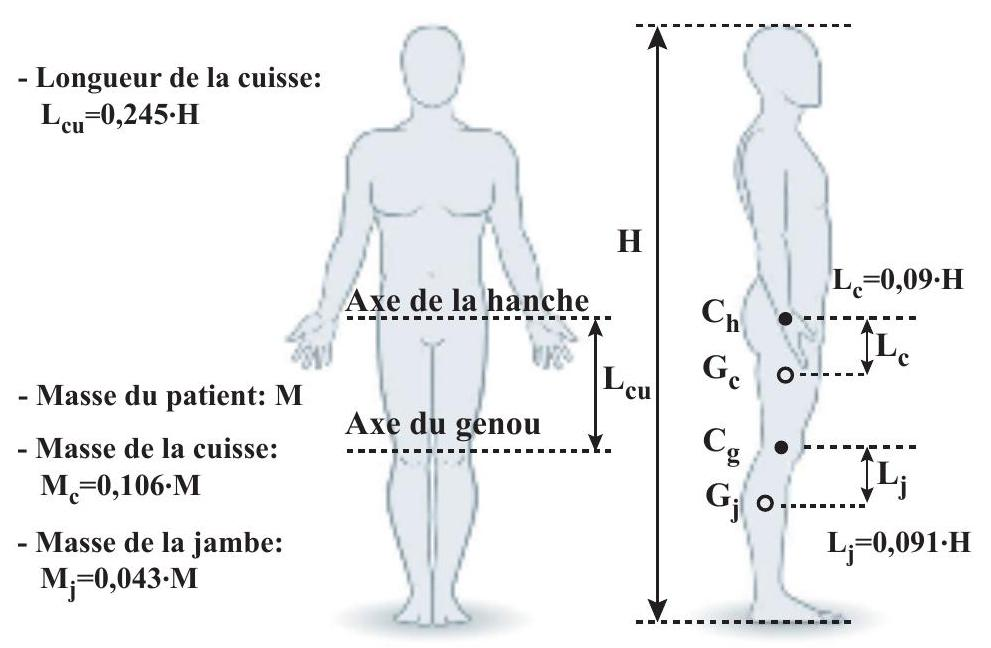
\includegraphics[max width=.7\textwidth]{2024_07_14_a83aebba33898893d39fg-12(1)}

\caption{\label{fig:ccs_mp_2024:fig:20}Patient de masse $M$ et de hauteur $H$}
\end{figure}

%Q 17. 
\question{\label{q:ccs_mp_2024:17}Déterminer l'expression de $\vec{V}_{G_{j}, 3 / 0}$ en fonction de $L_{c u}, L_{j}, \dot{\theta}_{4}, \dot{\theta}_{3}$ et de vecteurs unitaires du paramétrage.}

%Q 18. 
\question{\label{q:ccs_mp_2024:18}Exprimer la puissance $P_{p e s \rightarrow 3 / 0}$ de l'action mécanique de pesanteur sur 3 en fonction de $M_{j}, g, L_{j}$, $L_{c u}, \theta_{3}, \alpha_{3}, \theta_{4}, \dot{\theta}_{3}$ et $\dot{\theta}_{4}$.}

En procédant de façon similaire, la puissance développée par l'action mécanique de pesanteur sur la cuisse est $P_{\text {pes } \rightarrow 4 / 0}=M_{c} \cdot L_{c} \cdot g \cdot \cos \left(\theta_{4}\right) \cdot \dot{\theta}_{4}$.

La puissance totale développée par l'action mécanique de pesanteur sur la jambe et la cuisse est $P_{\text {pes }}=P_{\text {pes } \rightarrow 3 / 0}+$ $P_{\text {pes } \rightarrow 4 / 0}$. L'objectif est d'écrire cette puissance sous la forme $P_{\text {pes }}=C_{\text {pes }} \cdot \omega_{m}(t)$.

Dans le but de pouvoir continuer à mener l'étude à partir d'un modèle linéarisé de la motorisation, le couple $C_{\text {pes }}$ sera considéré comme constant (perturbation de type échelon), et sa valeur correspondra au cas le plus défavorable pour le système : patient dont la morphologie est la plus contraignante pour le système.

Le constructeur indique que le système peut supporter un patient de masse maximale 135 kg et une taille de $1,95 \mathrm{~m}$.

Dans ces conditions, $P_{p e s}=\left(K_{p 3} \cdot \cos \left(\theta_{3}-\alpha_{3}\right)+K_{p 4} \cdot \cos \left(\theta_{4}\right)\right) \cdot \dot{\theta}_{g}$ avec $K_{p 3}=3,42 \mathrm{~N} \cdot \mathrm{m}$ et $K_{p 4}=-34,12 \mathrm{~N} \cdot \mathrm{m}$. Il est rappelé que $\dot{\theta}_{g}(t)=a \cdot \dot{\lambda}(t), \dot{\theta}_{3}(t)=K_{3} \cdot \dot{\theta}_{g}(t)$ et $\dot{\theta}_{4}(t)=K_{4} \cdot \dot{\theta}_{g}(t)$ avec $a=4,25 \mathrm{rad} \cdot \mathrm{m}^{-1}, K_{3}=0,34$ (sans unité), $K_{4}=-0,66$ (sans unité), $K_{r}=\frac{1}{16}$ et $K_{v}=\frac{5 \cdot 10^{-3}}{2 \pi} \mathrm{m} \cdot \mathrm{rad}^{-1}$. De plus $\alpha_{3}=19,15^{\circ}$.

%Q 19. 
\question{\label{q:ccs_mp_2024:19}Exprimer $P_{\text {pes }}$ en fonction de $\theta_{3}, \alpha_{3}, \theta_{4}$ et $\omega_{m}(t)$.}

%Q 20. 
\question{\label{q:ccs_mp_2024:20}Lors de la flexion de genou sur un intervalle $\left[35^{\circ}, 85^{\circ}\right], \theta_{3}$ varie dans l'intervalle $\left[23,8^{\circ} ; 40,66^{\circ}\right]$ et $\theta_{4}$ dans l'intervalle $\left[-30,35^{\circ} ;-63,49^{\circ}\right]$, donner la valeur de $\theta_{3}$ et celle de $\theta_{4}$ pour lesquelles la valeur absolue du couple $C_{\text {pes }}$ est maximale.}

La valeur maximale de $\left|C_{\text {pes }}\right|$, trouvée avec ce qui précède, conduit à retenir $C_{\mathrm{pes}}=-0,005 \mathrm{~N} \cdot \mathrm{m}$. Suite à l'étude menée précédemment, il est possible de modéliser la commande du moteur selon la figure \ref{fig:ccs_mp_2024:fig:21}.

\begin{figure}[!h]\centering
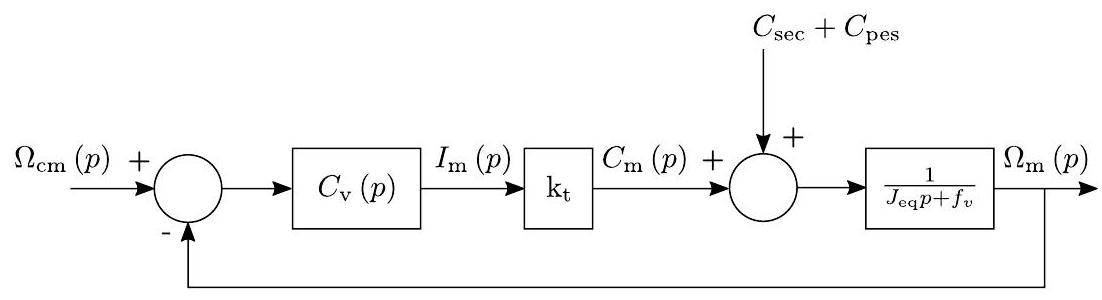
\includegraphics[max width=.7\textwidth]{2024_07_14_a83aebba33898893d39fg-13}

\caption{\label{fig:ccs_mp_2024:fig:21}Commande en vitesse angulaire du moteur}
\end{figure}
\subsubsection*{Quatrième essai en présence de la cuisse et de la jambe}
\paragraph*{— Conditions matérielles N°4}
Dans le but de valider la modélisation de la commande en vitesse du moteur, un essai est réalisé avec le système réel en plaçant des masses sur les berceaux, simulant la présence d'un patient dont la morphologie correspond à celle utilisée pour calculer $C_{\mathrm{pes}}$.

Il est rappelé que pour ce quatrième essai $C_{v}(p)=K_{p}$ avec $K_{p}=0,0094 \mathrm{~A} \cdot \mathrm{s} \cdot \mathrm{rad}^{-1}$ (valeur par défaut implantée dans la carte de commande).

\paragraph*{— Protocole de mesure N°4}
Une mesure de la vitesse angulaire du moteur $\omega_{m}(t)$ est réalisée pour une consigne en échelon de vitesse $\omega_{c m}(t)=\omega_{m 0}$ avec $\omega_{m 0}=285 \si{rad.s^{-1}}$ en partant de la position angulaire $\theta_{g}=35^{\circ}$.

Les conditions de mise en œuvre de ce quatrième essai sont résumées sur la figure \ref{fig:ccs_mp_2024:fig:22}.

\begin{figure}[!h]\centering
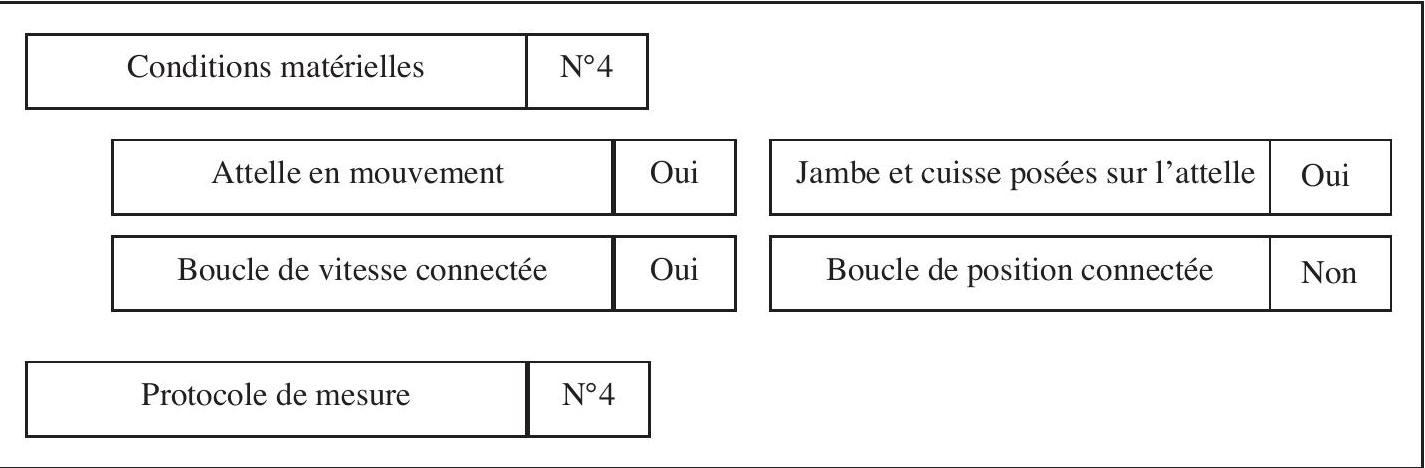
\includegraphics[max width=\textwidth]{2024_07_14_a83aebba33898893d39fg-13(1)}
\caption{\label{fig:ccs_mp_2024:fig:22}Résumé des conditions de mise en œuvre du quatrième essai}
\end{figure}
La figure \ref{fig:ccs_mp_2024:fig:23} montre :

\begin{itemize}
  \item une acquisition de $\omega_{m}(t)$ réalisée dans les conditions de mise en oeuvre résumées figure \ref{fig:ccs_mp_2024:fig:22} ;

  \item ainsi que le résultat de la simulation du modèle déterminé précédemment (figure \ref{fig:ccs_mp_2024:fig:21}).

\end{itemize}

Les performances attendues pour la commande en vitesse angulaire du moteur sont définies dans le tableau \ref{tab:ccs_mp_2024:02}.

\begin{table}[!h]
\centering
\begin{tabular}{llp{6cm}}
\hline
\textbf{Performance} & \textbf{Critère} & \textbf{Niveau} \\
\hline
Précision en vitesse angulaire & Erreur & Nulle en régime permanent pour une entrée en échelon \\
Rapidité & Temps de réponse à $5 \%$ & $t_{r 5 \%} \leqslant 0,3 \mathrm{~s}$ \\
\hline
\end{tabular}
\caption{\label{tab:ccs_mp_2024:02} Performances attendues de l'asservissement en vitesse du moteur de l'arthromoteur}
\end{table}



%Q 21. 
\question{\label{q:ccs_mp_2024:21}À partir de la figure \ref{fig:ccs_mp_2024:fig:21} et du tableau \ref{tab:ccs_mp_2024:02}, conclure sur la validité du modèle de la commande en vitesse angulaire du moteur en analysant l'écart simulé-mesuré. Par l'analyse de l'écart mesuré-souhaité, justifier que le correcteur $C_{v}(p)$ choisi par défaut ne convient pas. La réponse apportée doit être argumentée et s'appuyer sur des critères clairs et précis.}

Il apparait que le comportement du système réel n'atteint pas les performances attendues à cause de la présence de la jambe et de la cuisse sur l'attelle. Il est nécessaire de choisir et de dimensionner le correcteur $C_{v}$ pour que la commande en vitesse angulaire du moteur soit en accord avec les performances attendues du tableau \ref{tab:ccs_mp_2024:02}.

\subsubsection{Réglage du correcteur de la boucle de vitesse angulaire $C_{V}(p)$}
\begin{obj}
Régler les constantes du correcteur de la boucle de vitesse angulaire.
\end{obj}

La carte de commande choisie par le constructeur comporte un correcteur de type Proportionnel Intégral dont la fonction de transfert est $C_{v}(p)=K_{p}+\frac{K_{i}}{p}$. L'objectif est de déterminer la valeur de $K_{i}$ pour que la commande du moteur ait des performances au niveau de celles définies tableau \ref{tab:ccs_mp_2024:03} .

\begin{figure}[!h]\centering
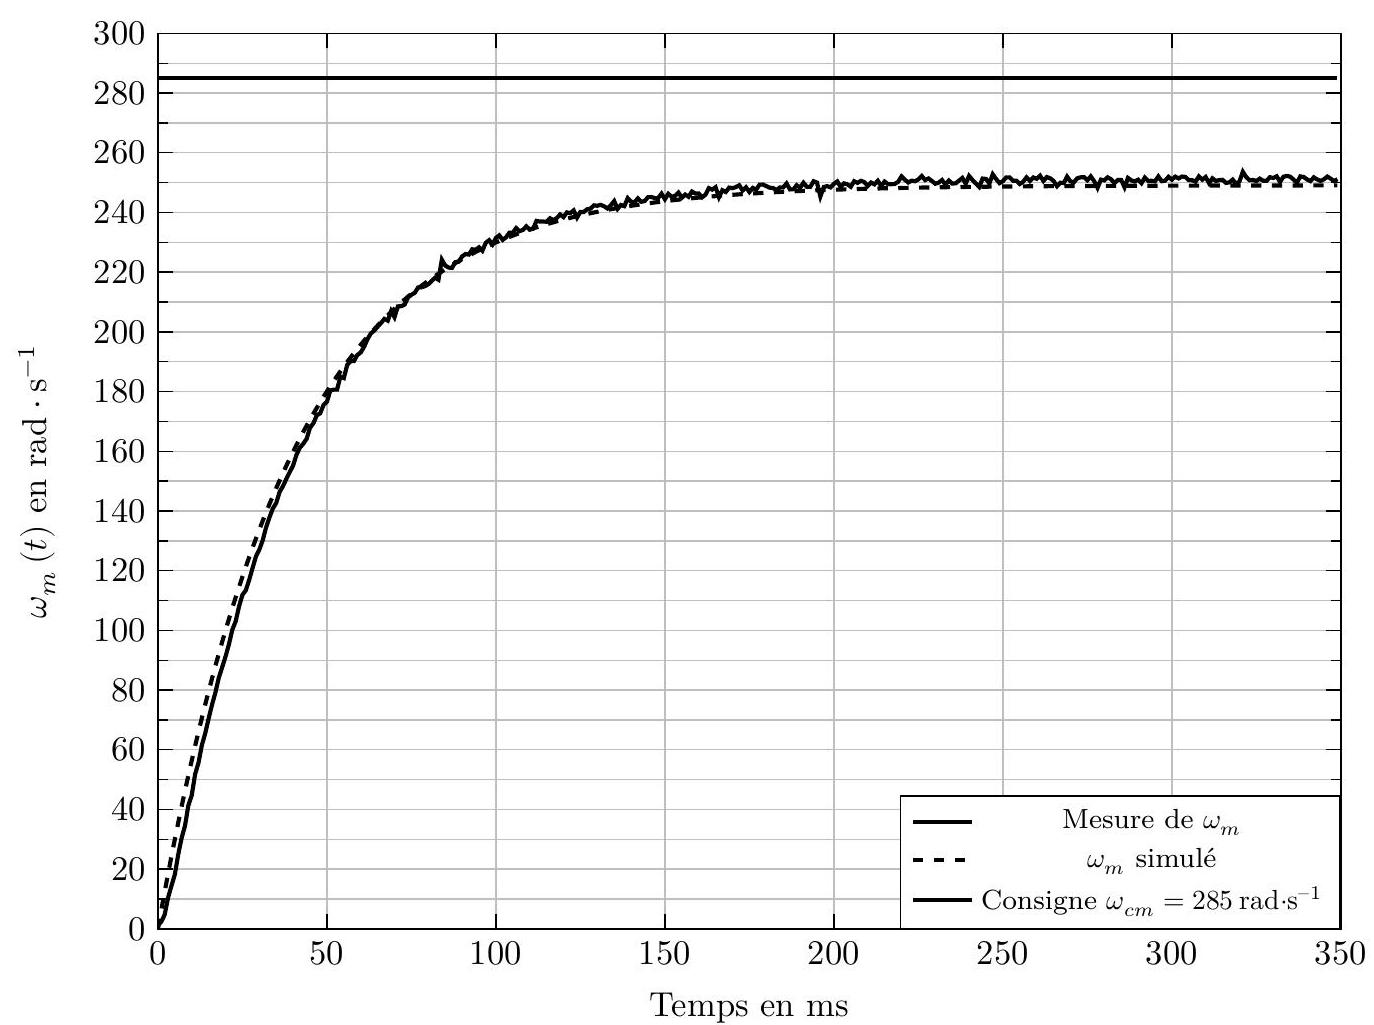
\includegraphics[max width=.7\textwidth]{2024_07_14_a83aebba33898893d39fg-14(1)}
\caption{\label{fig:ccs_mp_2024:fig:23}Mesure sur système réel et résultat de simulation pour une consigne de vitesse angulaire en échelon}
\end{figure}
\begin{figure}[!h]\centering
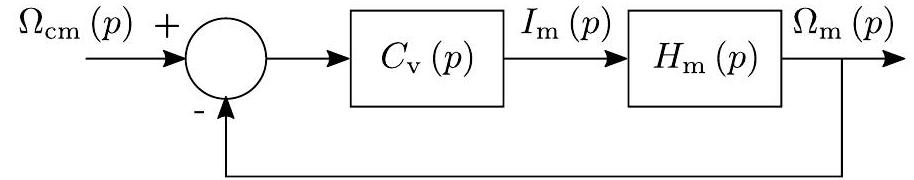
\includegraphics[max width=.5\textwidth]{2024_07_14_a83aebba33898893d39fg-14}
\caption{\label{fig:ccs_mp_2024:fig:24}Commande utilisée pour l'essai en consigne de vitesse angulaire du moteur}
\end{figure}

\subsubsection*{Données}

\begin{itemize}
  \item $H_{m}(p)=\frac{K_{m}}{1+\tau_{m} \cdot p}$ avec $K_{m}=10000 \si{rad.s^{-1}} \cdot \mathrm{A}^{-1}$ et $\tau_{m}=3,7 \mathrm{~s}$;

  \item il est rappelé que $K_{p}=0,0094 \mathrm{~A} \cdot \mathrm{s} \cdot \mathrm{rad}^{-1}$.

\end{itemize}

Le rôle du correcteur intégral est d'atténuer les effets de la perturbation. Les performances attendues pour la commande en vitesse angulaire du moteur sont définies dans le tableau tableau 3. Elles sont définies pour le cas le plus défavorable pour le système.

\begin{table}[!h]
\centering
\begin{tabular}{p{.25\linewidth}p{.5\linewidth}p{.25\linewidth}}
\hline
\textbf{Performance} & \textbf{Critère} & \textbf{Niveau} \\
\hline
Précision en vitesse angulaire & Erreur & Nulle en régime permanent pour une perturbation constante. \\
Amortissement & Chute de vitesse maximale pour une pertubation en échelon de $-0,005 \mathrm{~N} \cdot \mathrm{m}$, pendant la phase à vitesse constante & $\leqslant 14 \si{rad.s^{-1}} \cdot$ \\
Rapidité & Temps de réponse pour atteindre la vitesse en régime permanent à $\pm \SI{1}{rad.s^{-1}}$ en échelon de à $-0,005 \mathrm{~N} \cdot \mathrm{m}$ pendant la phase à vitesse constante. 
& $T_{r} \leqslant 0,3 \mathrm{~s}$ \\
\hline
\end{tabular}
\caption{\label{tab:ccs_mp_2024:03} Performances attendues de l'asservissement en vitesse angulaire du moteur de l'arthromoteur pour contrer les effets d'une perturbation}
\end{table}


%Q 22. 
\question{\label{q:ccs_mp_2024:22}Montrer que l'expression de $H_{v}(p)=\frac{\Omega_{m}(p)}{\Omega_{c m}(p)}$ peut se mettre sous la forme $H_{v}(p)=\frac{1+\tau \cdot p}{1+\frac{2 \xi}{\omega_{0}} p+\frac{p^{2}}{\omega_{0}^{2}}}$. Déterminer l'expression du facteur d'amortissement $\xi$ en fonction de $K_{p}, K_{m}, K_{i}$ et $\tau_{m}$. Quelle est l'influence de $K_{i}$ sur l'amortissement de la réponse à un échelon de consigne de vitesse angulaire ?}

%Q 23. 
\question{\label{q:ccs_mp_2024:23}À l'aide de la figure \ref{fig:ccs_mp_2024:fig:25}, choisir la valeur de $K_{i}$ qui permet à l'asservissement de vitesse angulaire du moteur de respecter tous les critères du tableau 3 sans dégrader l'amortissement de la réponse à un échelon de consigne de vitesse angulaire. Justifier ce choix.}

\begin{figure}[!h]\centering
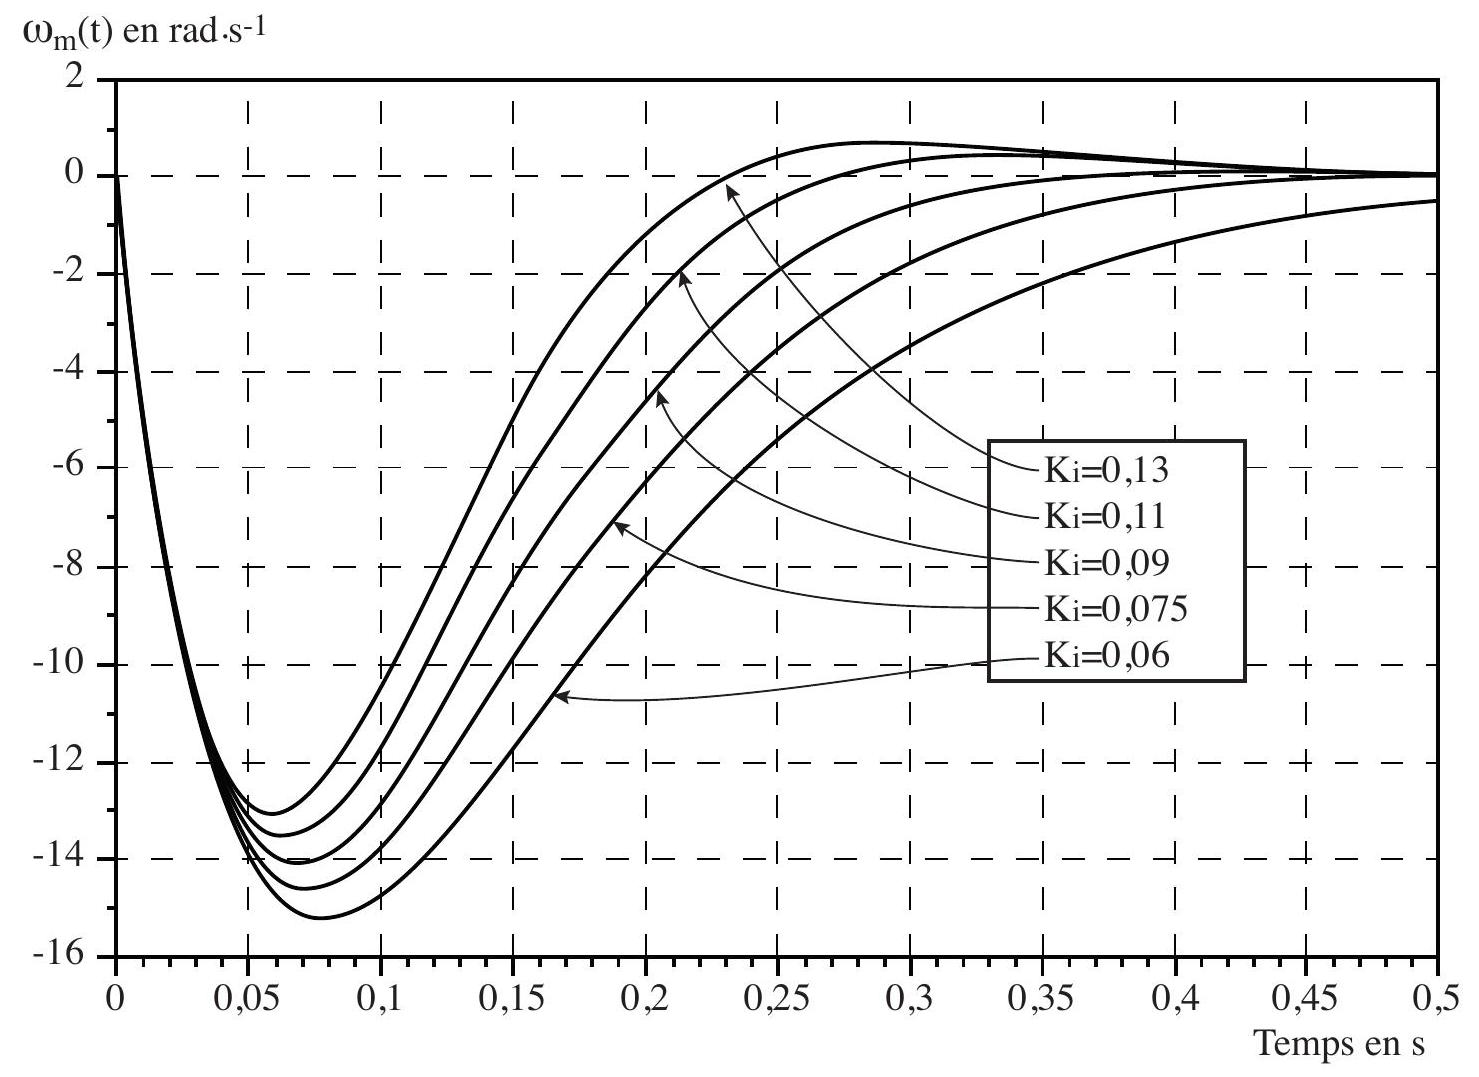
\includegraphics[max width=\textwidth]{2024_07_14_a83aebba33898893d39fg-15(1)}
\caption{\label{fig:ccs_mp_2024:fig:25}Chute de vitesse angulaire du moteur pour un échelon de perturbation de $-0,005 \mathrm{~N} \cdot \mathrm{m}$}
\end{figure}
La boucle d'asservissement du moteur étant totalement définie, il reste à étudier l'asservissement complet en position du genou.

\subsection{Réglage du correcteur de la boucle de position $C_{p}(p)$}

\begin{obj}
Régler les constantes du correcteur de la commande en position angulaire du genou.
\end{obj}

\begin{figure}[!h]\centering
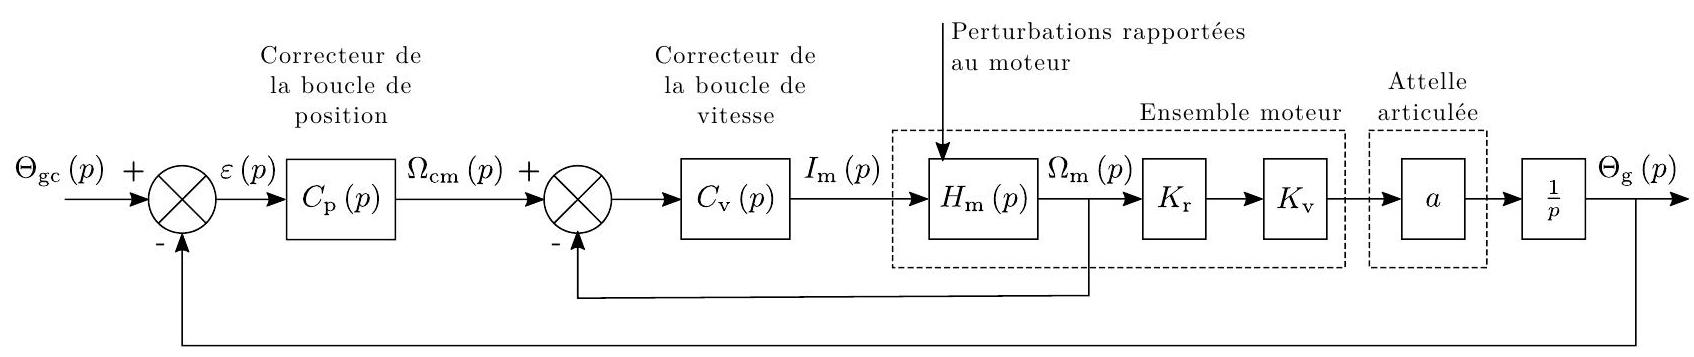
\includegraphics[max width=\textwidth]{2024_07_14_a83aebba33898893d39fg-15}
\caption{\label{fig:ccs_mp_2024:fig:26}Schéma-bloc de la commande en position du genou}
\end{figure}
L'objectif est maintenant de dimensionner le correcteur proportionnel $C_{p}(p)$ de la commande en position du genou implanté par le concepteur de l'arthromoteur. Le correcteur $C_{p}(p)$ est du type proportionnel avec $C_{p}(p)=$ $K_{g}$. La valeur par défaut de $K_{g}$ est $2865 \mathrm{~s}^{-1}$.

Il est essentiel que l'arthromoteur soit un bon «suiveur », et à ce titre l'exigence 1.2.1 doit être respectée pour assurer la qualité thérapeutique de l'arthromoteur.

Pour une consigne $\indice{\theta}{g c}(t)$ non constante, l'erreur $\varepsilon(t)=\theta_{g c}(t)-\theta_{g}(t)$ est inversement proportionnelle au gain de la F.T.B.O. $\indice{H}{bo}(p)=\frac{\Theta_{g}(p)}{\varepsilon(p)}$ qui est fonction de $K_{g}$. Un compromis entre la précision et la stabilité conduit à choisir $K_{g}$ tel que la pulsation de coupure $\omega_{0 B O}$ à 0 dB de la F.T.B.O. $\indice{H}{bo}(p)$ soit égale à $3 \si{rad.s^{-1}}$.

La figure \ref{fig:ccs_mp_2024:fig:27} représente une partie du diagramme de Bode en gain de la F.T.B.O. sur l'intervalle de pulsation $\left[0,1 \si{rad.s^{-1}} ; 10 \si{rad.s^{-1}}\right]$ pour $K_{g}=2865 \mathrm{~s}^{-1}$.

%Q 24. 
\question{\label{q:ccs_mp_2024:24}Déterminer la valeur de $K_{g}$ telle que la pulsation de coupure $\omega_{0_{B O}}$ de la F.T.B.O. $\indice{H}{bo}(p)$ soit égale à $3 \si{rad.s^{-1}}$.}


\begin{figure}[!h]\centering
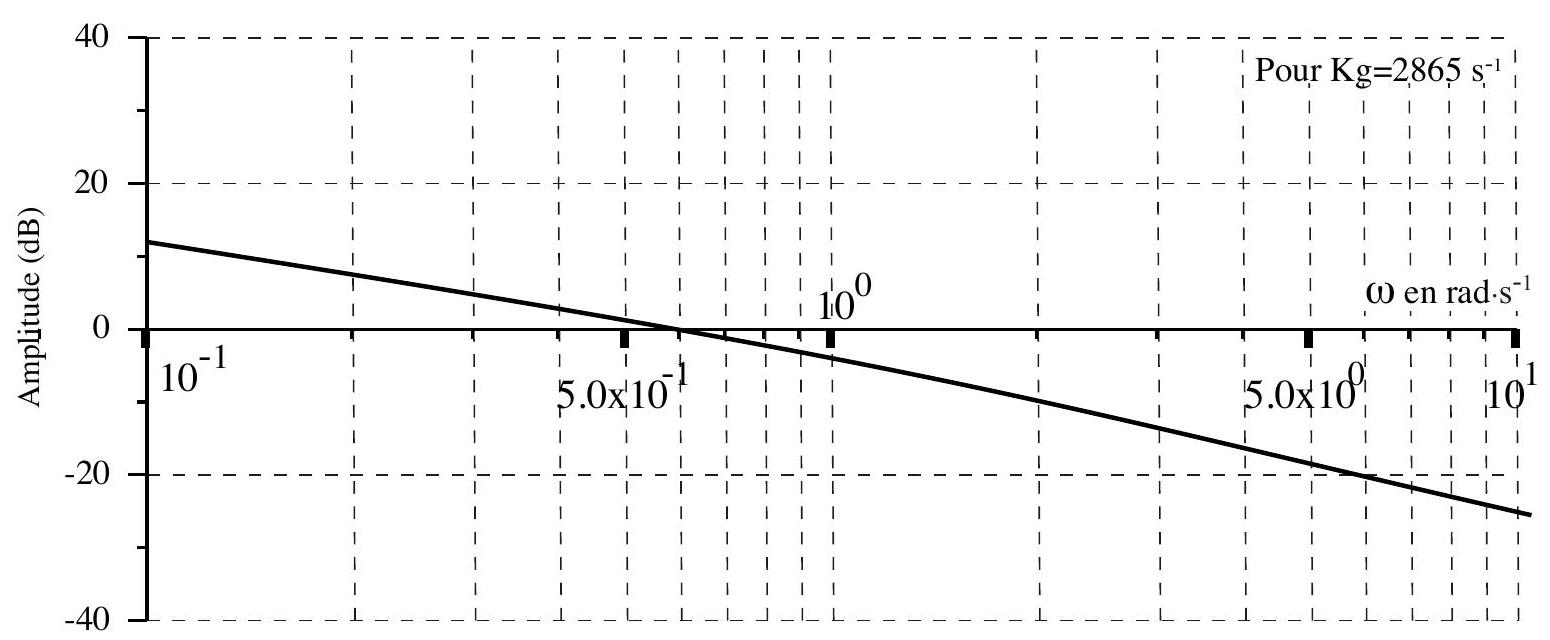
\includegraphics[max width=\textwidth]{2024_07_14_a83aebba33898893d39fg-16(1)}

\caption{\label{fig:ccs_mp_2024:fig:27}Diagramme de Bode en gain de la F.T.B.O de la commande en position angulaire du genou}
\end{figure}

Le correcteur de la commande en position du genou étant déterminé, il reste à valider la valeur de son gain $K_{g}$ en analysant le comportement du système réel vis-à-vis des exigences à respecter.

\section{Conclusion et synthèse}
\subsection{Validation des réglages de la carte de commande}

\begin{obj}
Valider les réglages théoriques à l'aide d'un essai sur l'arthromoteur.
\end{obj}

Suite à la détermination des paramètres du correcteur de la boucle de vitesse et de la génération de consigne, les valeurs trouvées dans les études précédentes sont implantées dans la carte de commande de l'arthromoteur. La figure \ref{fig:ccs_mp_2024:fig:29} représente le résultat d'un essai sur l'arthromoteur dans le cadre d'une rééducation des ligaments croisés. La consigne d'angle de genou impose une flexion de 35 degrés à 85 degrés.

\subsubsection*{Cinquième essai pour la validation du réglage du correcteur de la boucle de position du genou}

\subsubsection*{Conditions matérielles N°5}

Dans le but de valider la commande en position angulaire du genou, un essai est réalisé avec le système réel en présence d'un patient dont la morphologie correspond à celle utilisée pour calculer $C_{\mathrm{pes}}$.

\subsubsection*{Protocole de mesure N°5}
Une mesure de la position angulaire du genou $\theta_{g}(t)$ est réalisée pour une consigne angulaire $\indice{\theta}{g c}(t)$ du genou conforme au protocole de la rééducation des ligaments croisés, $\theta_{i}=35^{\circ}, \theta_{f}=85^{\circ}$ et $\omega_{0}=240^{\circ} \cdot \mathrm{min}^{-1}$.

\begin{figure}[!h]\centering
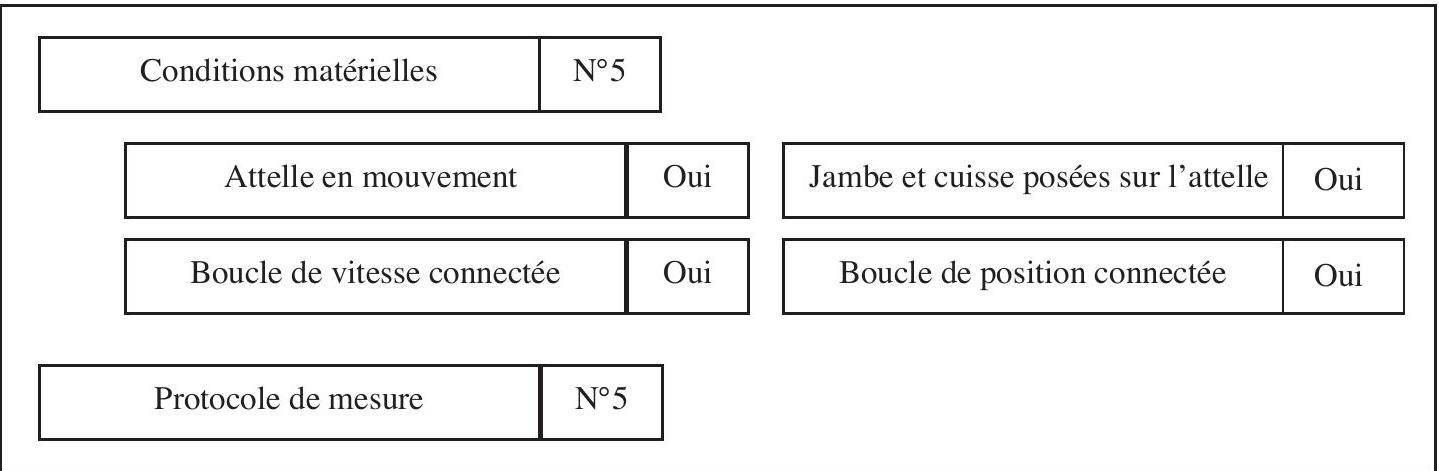
\includegraphics[max width=\textwidth]{2024_07_14_a83aebba33898893d39fg-16}
\caption{\label{fig:ccs_mp_2024:fig:28}Résumé des conditions de mise en œuvre du cinquième essai}
\end{figure}

%Q 25. 
\question{\label{q:ccs_mp_2024:25}Les exigences 1.2.1 et 1.2.3 sont-elles respectées par l'arthromoteur automatisé suite aux réglages du correcteur de la boucle de vitesse et du gain $K_{g}$ du correcteur de la boucle de position? Argumenter avec des comparaisons quantifiées.}

\begin{figure}[!h]\centering
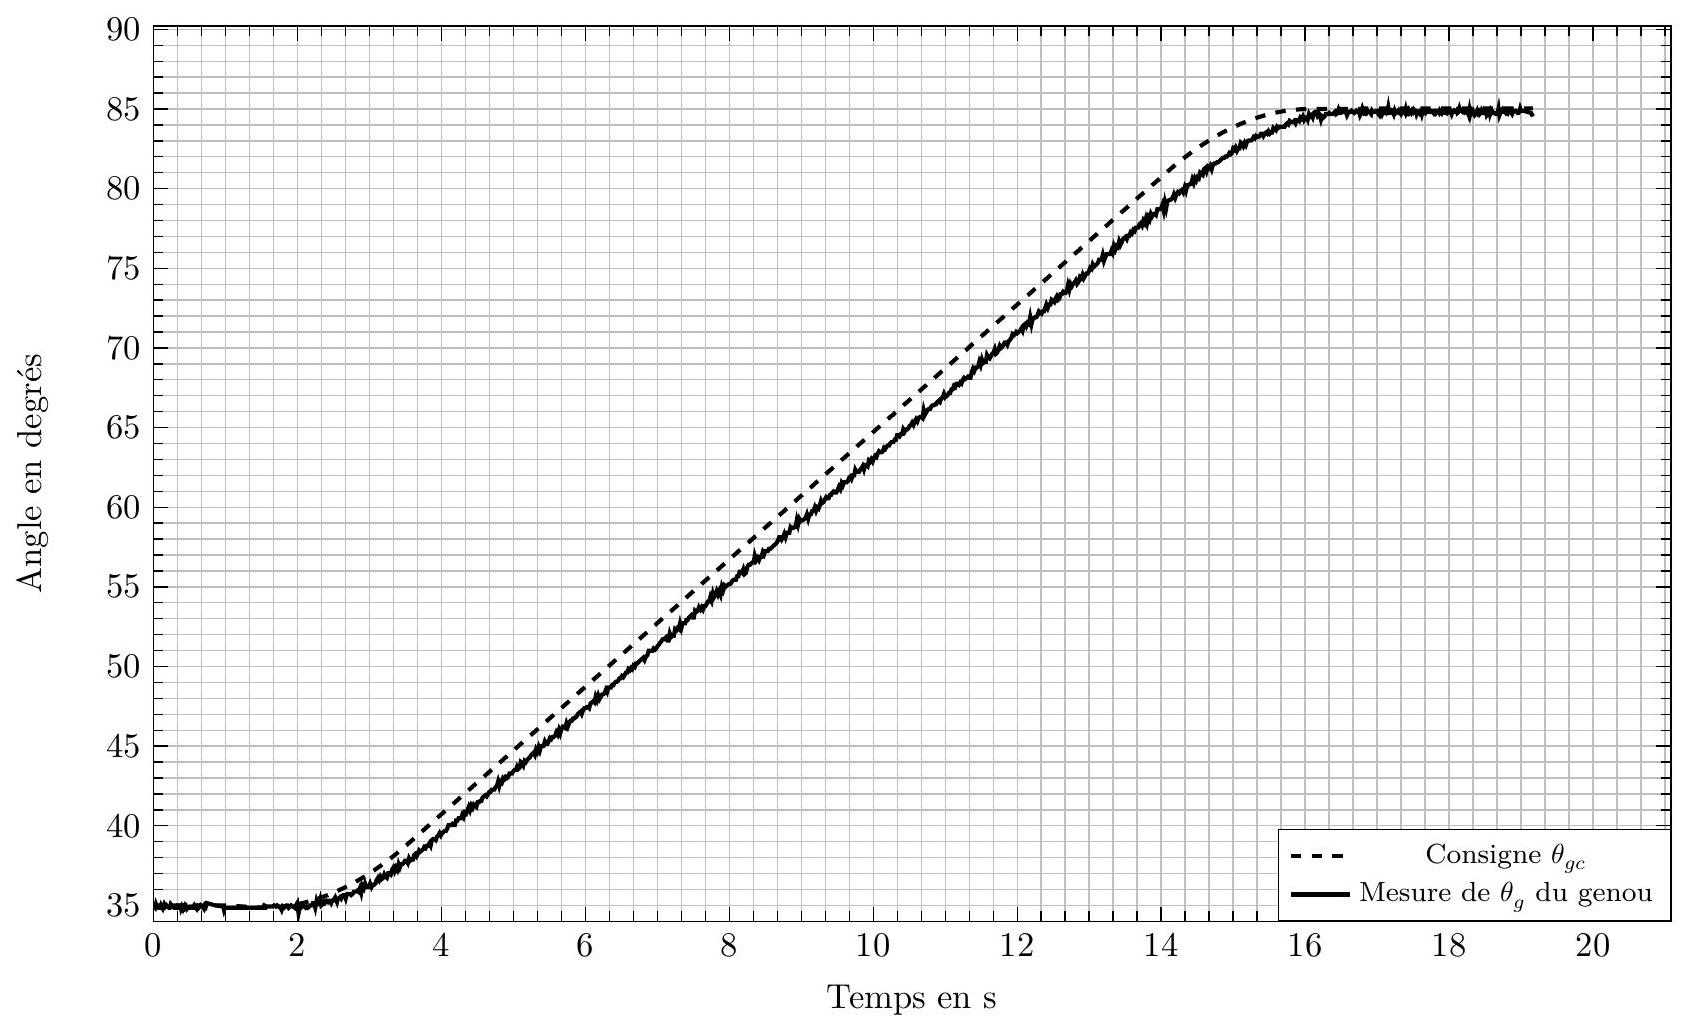
\includegraphics[max width=\textwidth]{2024_07_14_a83aebba33898893d39fg-17}
\caption{\label{fig:ccs_mp_2024:fig:29}Essai réalisé avec l'arthromoteur automatisé réglé}
\end{figure}
\subsection{Synthèse de l'étude}

\begin{obj}
Conclure sur la capacité de l'arthromoteur automatisé à être qualifié pour tout type de rééducation passive du genou avec les paramètres caractéristiques de la carte de commande déterminés dans l'étude précédente.
\end{obj}

L'étude réalisée dans ce sujet avait pour contexte la rééducation des ligaments croisés du genou. Cependant, l'arthromoteur permet d'atteindre des angles limites de $-5^{\circ}$ et $110^{\circ}$ (figure \ref{fig:ccs_mp_2024:fig:30}) et un choix de vitesses angulaires du genou de 50 à $240^{\circ}$ par minute pour couvrir plusieurs types de rééducation du genou. Il est nécessaire de vérifier si le réglage de l'arthromoteur automatisé, effectué précédemment, reste valable pour tout type de fonctionnement en mode passif.

Toutefois, cette réflexion sera limitée au cas où la plage $\left(\theta_{f}-\theta_{i}\right)$ resterait constante et égale à $50^{\circ}$ et où le mouvement de flexion-extension serait choisi pour d'autres valeurs de $\theta_{i}, \theta_{i} \in\left[-5^{\circ}, 60^{\circ}\right]$.

%Q 26. 
\question{\label{q:ccs_mp_2024:26}Le modèle adopté pour le réglage des deux correcteurs de la commande de l'arthtomoteur automatisé est un modèle linéaire. Quel paramètre du modèle de la figure \ref{fig:ccs_mp_2024:fig:26}, choisi constant pour cette étude, est affecté par le choix de $\theta_{i}, \theta_{i} \in\left[-5^{\circ}, 60^{\circ}\right]$ ?}

%Q 27. 
\question{\label{q:ccs_mp_2024:27}Citer deux autres grandeurs physiques de la figure \ref{fig:ccs_mp_2024:fig:26} qui sont fonction de ce paramètre et indiquer si l'étude effectuée prend en compte cette variation.}

%Q 28. 
\question{\label{q:ccs_mp_2024:28}Parmi les deux correcteurs de la commande, lequel aurait son réglage affecté par la variation de ce paramètre? Justifier succinctement cette réponse.}

\begin{figure}[!h]\centering
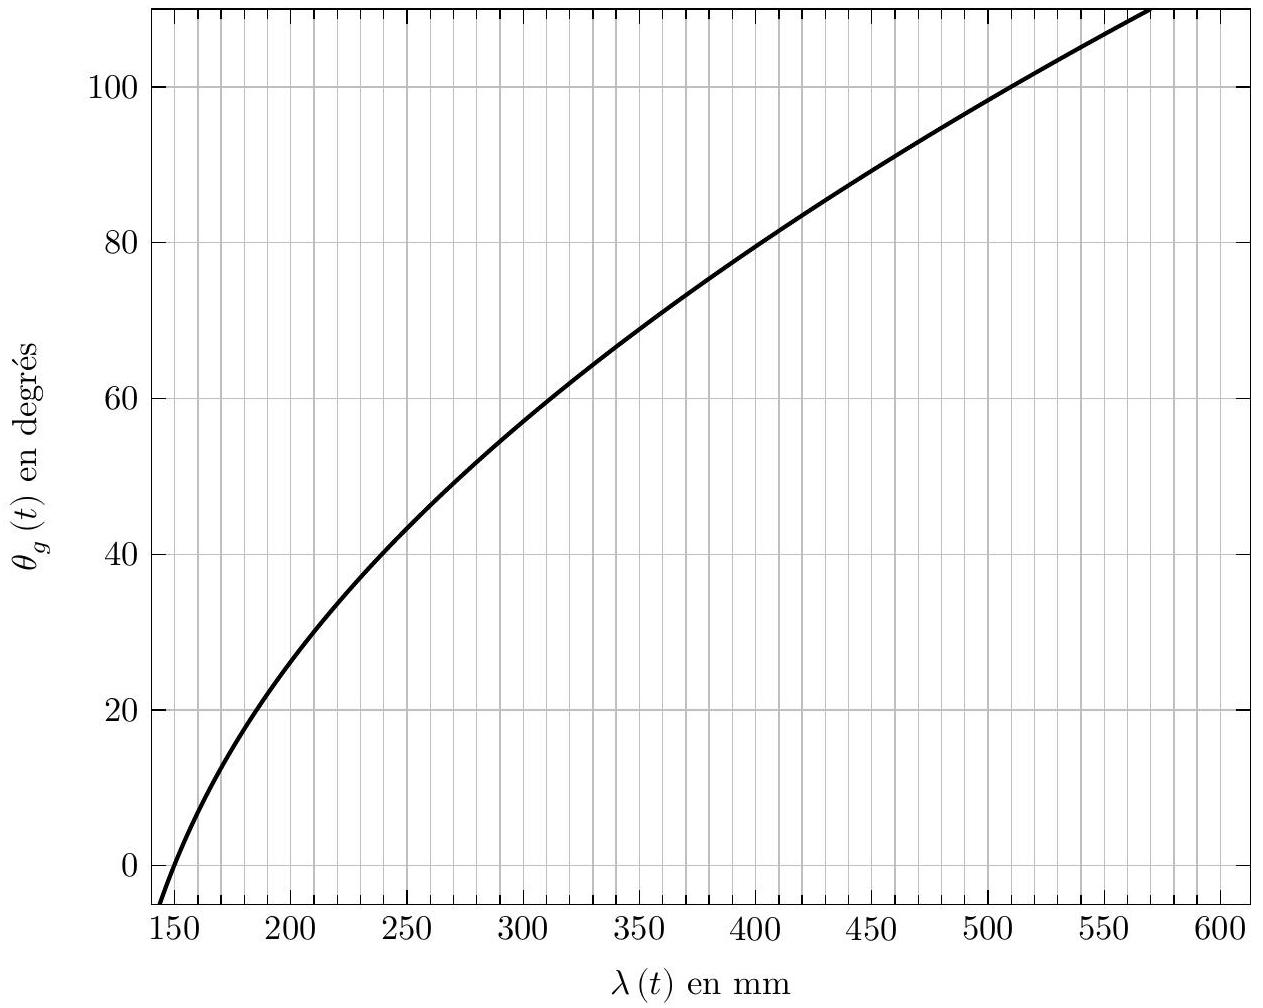
\includegraphics[max width=\textwidth]{2024_07_14_a83aebba33898893d39fg-18}
\caption{\label{fig:ccs_mp_2024:fig:30}Angle du genou en fonction du déplacement de la coulisse 2 pour toute la plage d'utilisation}
\end{figure}

\clearpage
\newpage

\section{Annexes}
\subsection{Diagramme des exigences de l'arthromoteur pour la rééducation des ligaments croisés}

\begin{figure}[!h]\centering
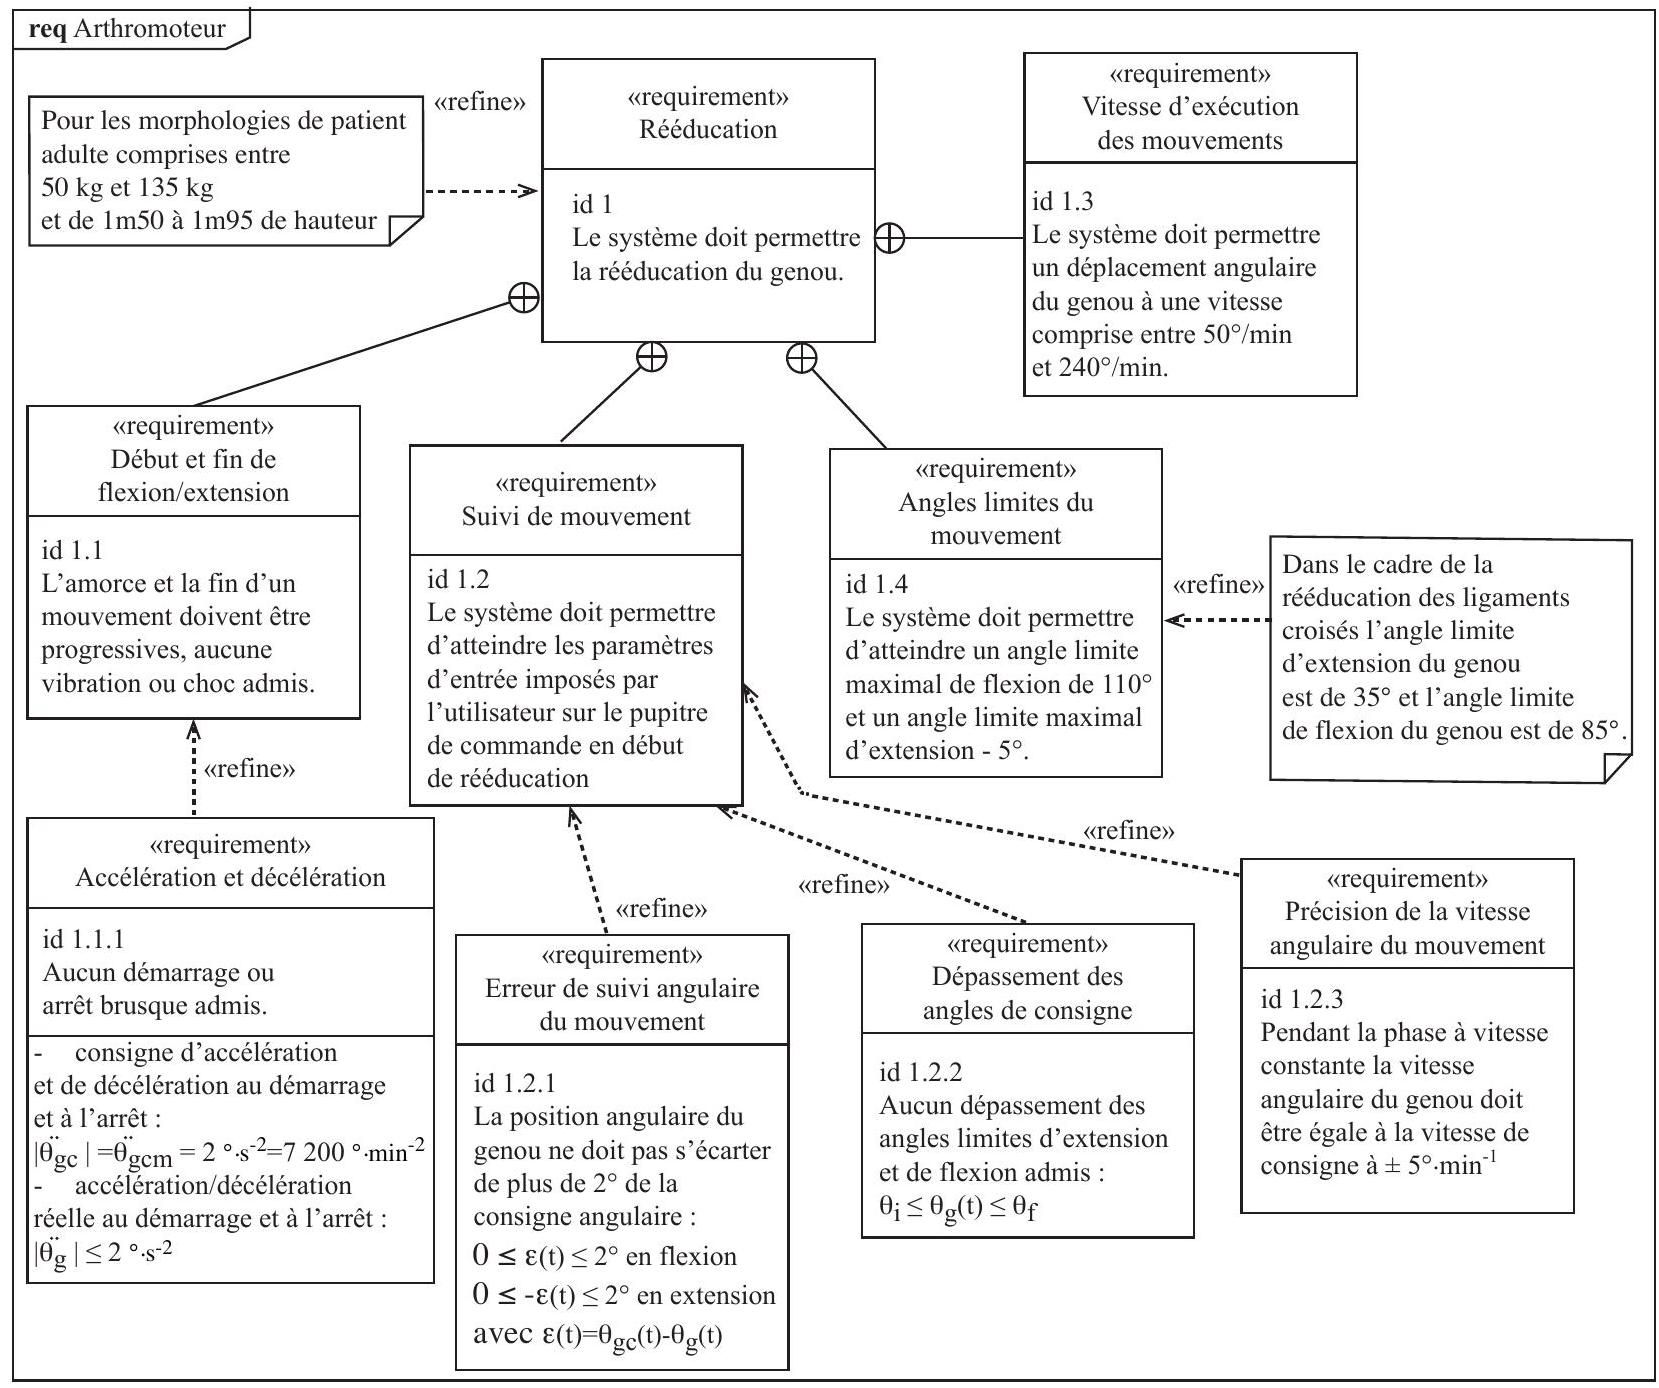
\includegraphics[max width=\textwidth]{2024_07_14_a83aebba33898893d39fg-19}
\caption{\label{fig:ccs_mp_2024:fig:31}Exigences liées à la rééducation des ligaments croisés du genou}
\end{figure}

\newpage

\subsection{Diagramme BDD de l'arthromoteur}
\begin{figure}[!h]\centering
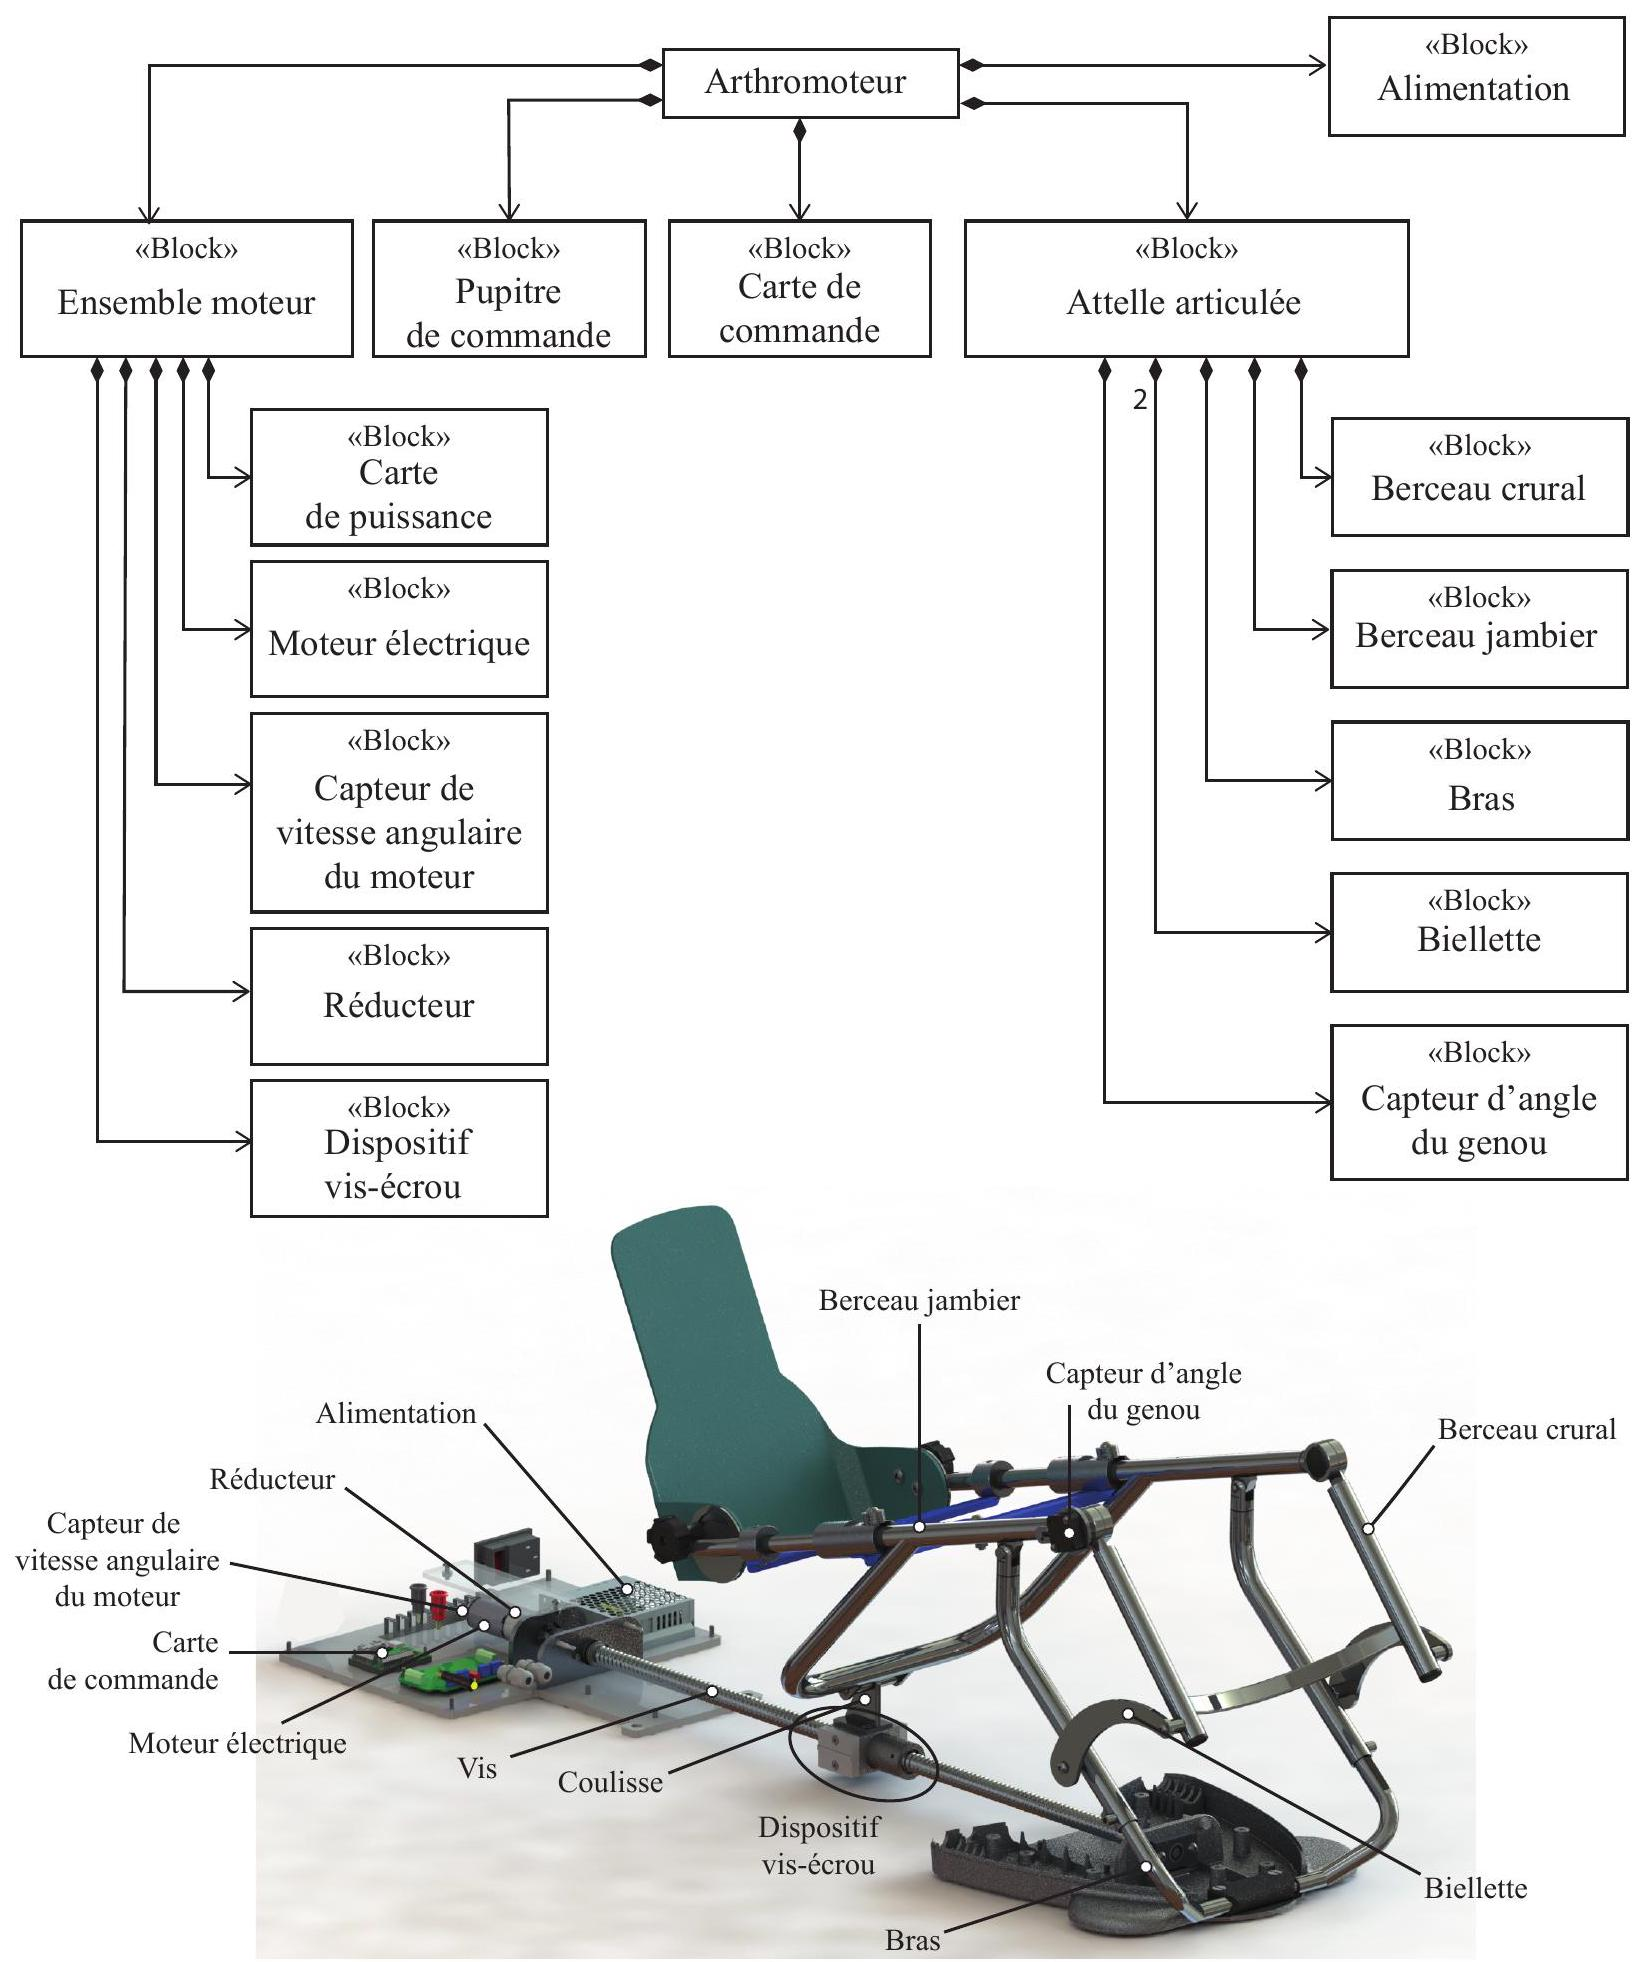
\includegraphics[max width=\textwidth]{2024_07_14_a83aebba33898893d39fg-20}
\caption{\label{fig:ccs_mp_2024:fig:32}Diagramme BDD de l'arthromoteur automatisé}
\end{figure}
\newpage

\section{Description des chaines d'information et de puissance de l'arthromoteur automatisé}

\begin{figure}[!h]\centering
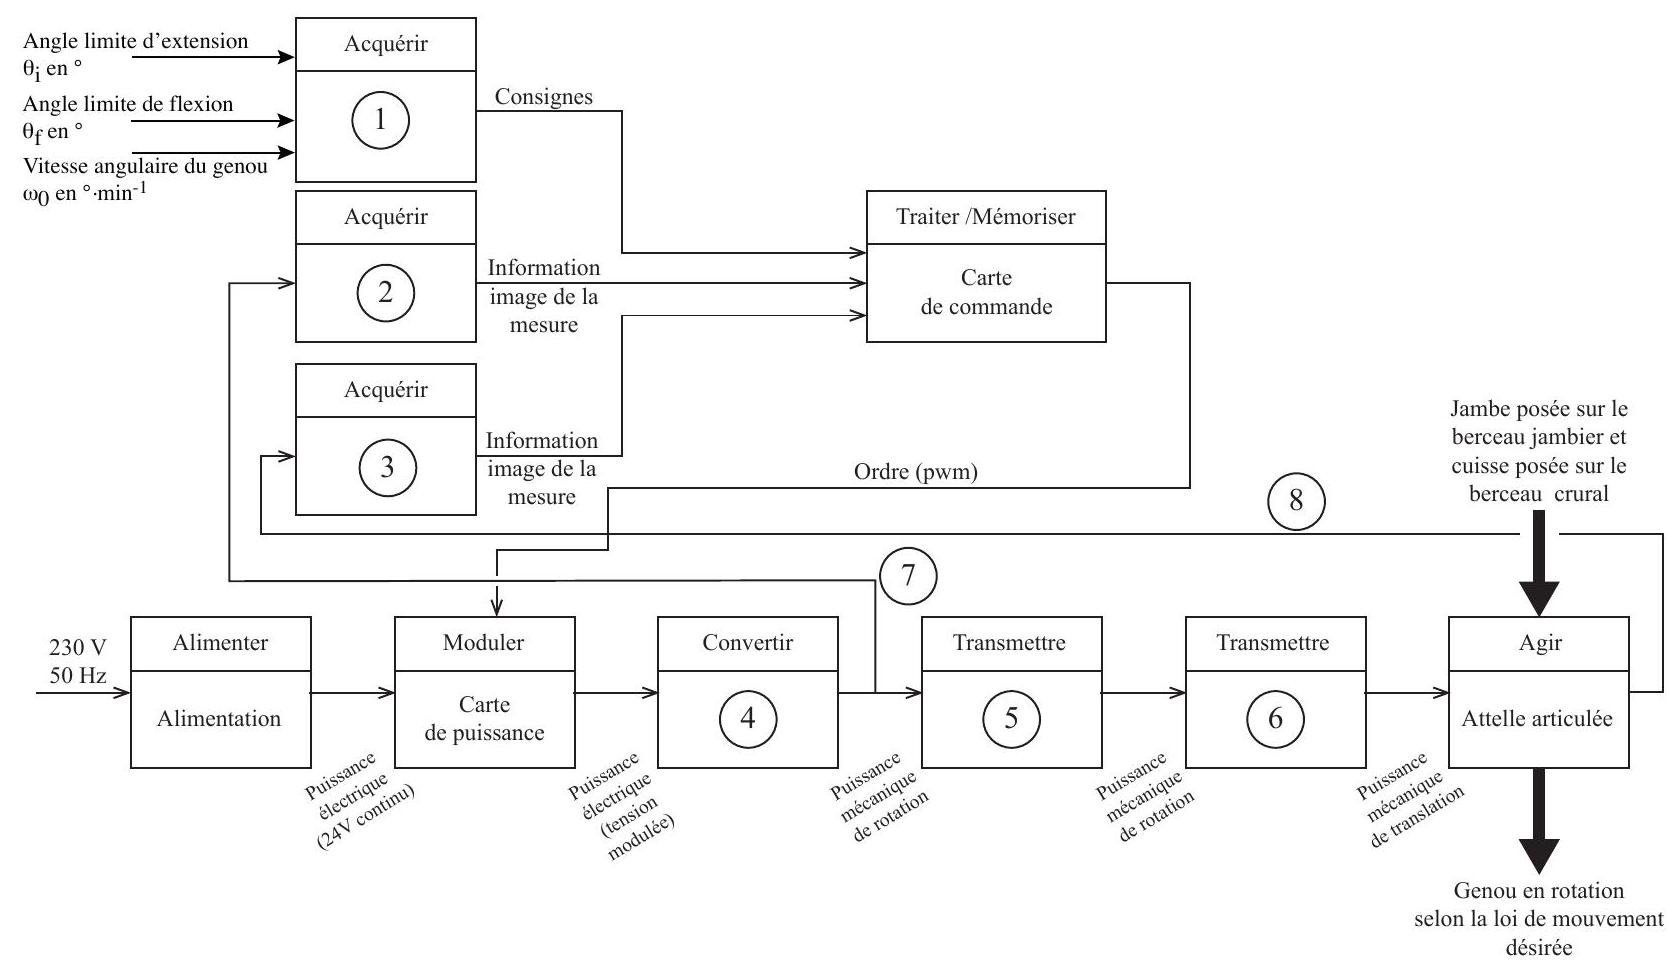
\includegraphics[max width=\textwidth]{2024_07_14_a83aebba33898893d39fg-21}
\caption{\label{fig:ccs_mp_2024:fig:33}Chaines d'information et de puissance de l'arthromoteur automatisé}
\end{figure}
